\documentclass[twoside,openright]{xduugthesis}

\usepackage{float}

\xdusetup{
  style / font-type = font,
  style / latin-font = tacn,
  style / cjk-font = fandol,
  info / title = {基于大语言模型的算法伪代码自动注释与示例代码生成系统设计与实现},
  info / author = {张迪},
  info / department = {计算机科学与技术学院},
  info / major = {软件工程},
  info / supervisor = {蔺一帅},
  info / class-id = {2203053},
  info / student-id = {22009201038},
  info / abstract = {abstract-zh.tex},
  info / abstract* = {abstract-en.tex},
  info / keywords = {大语言模型；伪代码；代码注释生成；代码生成；提示词工程；Spring AI},
  info / keywords* = {Large Language Models; Pseudocode; Code Comment Generation; Code Generation; Prompt Engineering; Spring AI},
  info / bib-resource = {references.bib}
}

\begin{document}

\chapter{绪论}

\section{研究背景}

算法伪代码（Pseudocode）是一种介于自然语言与程序设计语言之间的算法描述方式，广泛运用于计算机科学教材、学术论文、技术文档以及算法竞赛题解中。它通过简化的语法结构、通用的控制流关键词（如IF、FOR、WHILE）以及自然语言辅助说明，使算法逻辑更加清晰易懂，同时避免了具体编程语言（如C++、Java、Python）的语法细节对算法思想的干扰。因此，伪代码成为算法教学、科研交流与工程设计中表达算法的主流工具之一。

然而，伪代码的自由度和非标准化特征也带来了明显的理解和实现障碍。一方面，初学者往往缺乏足够的算法阅读训练，难以准确理解伪代码中隐含的变量类型、边界条件、递归基例以及复杂控制流之间的语义关系；另一方面，开发者和研究人员在阅读伪代码后，通常需要手工将其转换为可运行的源代码。这一过程不仅耗时、易错，而且难以保证转换结果与原始算法逻辑的一致性。尤其是在快速原型开发或跨语言实现场景下，伪代码到实际代码的映射成本显著增加了开发负担。

随着人工智能技术的快速发展，大语言模型（Large Language Models, LLMs）在自然语言处理和代码生成领域展现出突破性能力。以GPT系列、Code Llama、StarCoder、DeepSeek Coder等为代表的模型，通过在海量文本与代码语料上的预训练，具备了出色的语义理解、代码补全、代码生成甚至代码调试能力。GitHub Copilot、Cursor等智能编程助手已证明，LLMs能够根据自然语言注释或部分代码片段生成高质量的完整代码，极大地提升了软件开发的效率。这些进展为解决伪代码理解与转换问题提供了新的技术路径。

基于上述背景，本课题的目标是设计并实现一个面向算法教学与工程辅助的智能系统，该系统能够以算法伪代码作为输入，自动完成以下两项核心任务，并提供稳定、易用的交互方式：

自动生成详细、准确的中文语义注释：系统应能够分析伪代码的语法结构、识别关键变量和控制流，在保留原始伪代码框架的基础上，为每一行或每一个逻辑块生成解释其意图的中文注释。注释应涵盖变量的作用、循环的边界条件、分支判断的逻辑依据以及函数或递归调用的含义，使阅读者能够像阅读带有旁注的教材一样快速理解算法思想。

自动生成可执行的目标代码：系统应能够将相同伪代码转换为符合指定编程语言（当前版本支持Python和Java）语法规范、风格统一、可直接运行（或经微小调整即可运行）的示例代码。生成的代码应尽量保留伪代码中的变量命名和结构体，并包含必要的边界处理及输入输出示例，以帮助用户快速验证算法正确性或嵌入到实际项目中。

基于上述背景，本课题期望交付一个可交互的Web原型系统，用户可以直接在线提交伪代码，并实时获得带注释的伪代码和示例代码。该系统可以服务于计算机专业的学生与教师，辅助算法教学与自学；也可用于软件工程中的原型开发，帮助开发者快速从算法描述过渡到可运行代码。通过将大语言模型的能力引入伪代码处理这一传统需求场景，本课题旨在降低算法学习的门槛，提高从算法思想到代码实现的转化效率，并为后续的智能编程辅助工具研究提供实践参考。

\section{国内外研究现状}
\subsection{代码注释自动生成}
代码注释生成是软件工程与自然语言处理交叉领域的重要研究方向。早期方法主要基于规则与模板：通过匹配关键词、函数名等信息，利用预定义模板生成注释。这类方法简单直接，但灵活性差，难以处理复杂逻辑[1]。随后出现了基于抽象语法树的方法：通过解析代码结构，提取语法节点特征，结合序列到序列（Seq2Seq）模型生成注释[2]。这类方法能更好地理解代码逻辑，但对语法解析工具依赖性较强。

随着深度学习的发展，基于Transformer架构的注释生成成为主流。特别是预训练模型如CodeBERT、CodeT5等在代码摘要任务上表现优异[3]。近年来，以GPT为代表的大语言模型凭借其强大的上下文理解能力，在代码注释生成任务上取得了突破性进展，能够生成更加自然、语义丰富的注释[4]。
\subsection{代码自动生成}
代码自动生成旨在根据高层描述生成可执行代码。基于模型驱动架构的方法通过定义平台无关模型到平台相关模型的转换规则来生成代码，在特定领域有效，但需要复杂的建模过程[5]。基于程序合成的方法通过形式化规约或输入输出示例在程序空间中搜索目标代码，理论严谨但搜索空间巨大。

基于深度学习的代码生成将任务视为序列生成问题，使用神经网络学习从自然语言描述到代码序列的映射。GPT-4、GitHub Copilot等已成为当前最先进的代码生成工具，能够生成高质量、多语言的代码片段。研究也表明，LLMs在教育领域具有辅助学习的潜力[6]。
\subsection{大语言模型在结构化任务中的应用}
如何引导大语言模型生成结构化输出是当前研究热点。思维链（Chain-of-Thought）方法通过让模型生成中间推理步骤，显著提升了逻辑推理能力[7]。程序引导（Program-aided）方法要求模型生成可执行程序来处理复杂任务。此外，通过在提示词中明确输出格式（如JSON、XML）或使用输出解析器后处理，可以获得结构化数据。
\subsection{伪代码处理相关研究}
专门针对伪代码自动处理的研究相对较少。早期工作多基于定义严格的伪代码语法构建转换器，对输入要求高，实用性有限。大语言模型的出现为此提供了新途径，其强大的泛化能力可以理解混合自然语言和简单代码结构的文本。在教育领域，有工具尝试可视化伪代码执行，但“注释生成+代码生成”直接服务于理解与实现环节的端到端系统仍不多见。
\subsection{研究现状总结与本课题定位}
综上，现有研究存在以下不足：（1）传统方法对伪代码语法依赖性过强，难以处理非标准化输入；（2）基于深度学习的方法需要大量标注数据，迁移成本高；（3）针对算法伪代码这一特定形式，缺乏端到端、可交互的实用系统。本课题定位于：利用大语言模型的泛化能力，结合轻量级预处理和提示词工程，设计实现一个面向教学和工程场景的伪代码自动注释与代码生成系统。
\section{研究目的与意义}
研究目的：设计并实现一个基于大语言模型的智能系统，能够对输入的算法伪代码进行语义分析，生成详细的行间/行内中文注释，并进一步生成可执行的目标代码（Python/Java）。具体目标包括：（1）构建端到端的伪代码理解与生成系统；（2）设计轻量级预处理模块提取关键结构信息；（3）研究面向两个子任务的有效提示词工程方法；（4）构建测试数据集并进行量化评估。

理论意义：拓展大语言模型在非标准化、半结构化文本语义解析中的应用场景；推动提示词工程在结构化输出生成中的方法论研究；丰富代码生成与注释生成的评价体系。

实践意义：为教师和学生提供快速将伪代码转化为带注释代码的工具，降低学习门槛，提升教学效率；辅助工程原型快速开发；促进代码文档的自动化与智能化；为Spring Boot+Spring AI的工程化集成提供技术示范。。

\section{本文的组织结构}
本文共分七章。第一章绪论阐述研究背景、现状、目的意义；第二章介绍相关技术；第三章进行系统需求分析；第四章阐述系统总体设计；第五章详细描述各模块实现；第六章报告测试与评估结果；第七章总结全文并展望未来工作。

\chapter{相关技术概述}
本章主要对基于 SpringAI的伪代码注释和实例代码生成系统所涉及的相关技术进行介绍，为后续系统需求分析、概要设计和详细实现提供技术基础。本章按照系统所采用的主要技术进行介绍。

\section{Spring AI框架}
Spring AI是Spring生态中用于集成人工智能模型的框架，提供了统一的API接口来调用不同大语言模型。其核心组件包括：

ChatClient：同步调用大语言模型的核心客户端，支持消息角色（system、user、assistant）管理。

StreamingChatClient：异步流式调用客户端，适用于需要实时逐字输出的场景。

PromptTemplate：支持占位符替换的提示词模板，可从外部文件加载模板内容。

ChatOptions：模型参数配置，如temperature（控制生成随机性）、maxTokens（最大输出长度）等。

本系统选择Spring AI的主要原因是其与Spring Boot生态无缝集成，配置简洁，技术新颖且支持多模型同时配置。

\section{大语言模型API}
本系统选用两款大语言模型作为后端服务：

DeepSeek Coder：由深度求索公司推出的代码专用大语言模型，在代码生成和补全任务上表现优异，成本较低。本系统将其作为默认模型。

OpenAI GPT-4：性能顶尖的通用模型，代码理解能力强，但成本较高，用作备用模型在DeepSeek限流或失败时自动切换。

两款模型均通过HTTP API调用，本系统使用Spring AI的ChatClient进行封装。
\section{提示词工程}
提示词工程（Prompt Engineering）是指通过设计输入提示词来引导大语言模型输出符合预期的结果。常用的策略包括：

指令式（Zero-shot）：直接给出任务描述和输出格式要求，不提供示例。适用于简单任务。

少样本示例式（Few-shot）：在提示词中提供若干正确示例，模型模仿示例风格输出。适用于需要控制输出格式和风格的场景。

思维链（Chain-of-Thought）：要求模型先给出推理步骤再输出最终答案，适用于复杂逻辑任务。

本系统针对“注释生成”和“代码生成”两个任务，结合指令式和少样本示例式设计提示词模板，并输出格式约束（如要求用```包围代码块）。

\section{代码格式化工具}
为保证生成代码的可读性和风格一致性，本系统在后处理阶段集成了两款代码格式化工具：

autopep8：Python代码自动格式化工具，遵循PEP 8规范。

google-java-format：Google开源的Java代码格式化工具，统一Java代码风格。

这些工具通过命令行调用，对LLM生成的原始代码进行格式化后输出。


\chapter{系统需求分析}
本章主要对基于 JavaWeb 和 LaTeX 的学术论文智能排版系统进行需求分析。该系统面向高校学生及具有论文写作需求的用户，主要目标是通过 Web 平台降低 LaTeX 使用门槛，提高论文编辑、模板使用、编译预览和错误排查效率。系统围绕论文写作与排版流程展开，主要包括用户管理、论文项目管理、模板管理、LaTeX 在线编辑、论文编译、编译错误分析和 AI 对话辅助等功能。

需求分析是系统设计与实现的基础。通过明确系统功能性需求和非功能性需求，可以为后续概要设计、数据库设计和详细实现提供依据。本章将结合系统实际功能，对各模块需求进行分析。

\section{系统目标与范围}
本系统面向算法教学场景，目标用户为计算机专业学生、教师以及需要快速理解算法逻辑的软件开发人员。系统接收非标准化的算法伪代码文本作为输入，自动生成以下两类输出：（1）在原伪代码基础上添加详细、准确的中文行间/行内注释；（2）根据伪代码逻辑生成Python或Java语言的可执行示例代码。

系统暂不处理任意复杂领域特定的伪代码，聚焦于教学场景中常见的经典算法（排序、查找、递归、动态规划基础等）和控制结构（顺序、分支、循环）。

\subsection{功能性需求}
系统功能性需求以用例图形式呈现，核心用例包括：

伪代码预处理：用户输入伪代码后，系统自动执行文本清洗（去除无关字符、统一关键词）、结构识别（基于缩进和关键词）、变量名提取，输出半结构化中间表示。

自动生成注释：用户可选择仅生成注释，系统基于预处理结果调用LLM，返回带注释的伪代码。注释应解释每行或每段代码的意图，包括变量含义和操作目的。

自动生成代码：用户可选择目标语言（Python/Java），系统调用LLM生成符合该语言语法规范、风格统一的示例代码。

结果展示与导出：系统在Web界面语法高亮显示生成结果，支持一键复制和下载为文件。

每个用例均包含基本流程、备选流程（如API调用失败时的降级提示）和异常处理。\begin{figure}
    \centering
    
\includegraphics[width=0.5\linewidth]{project_16_367403ad.jpg}
    \caption{签名}
    \label{fig:placeholder}
\end{figure}


\subsection{非功能性需求}
响应时间：简单伪代码（≤10行）≤5秒，复杂伪代码（>10行或含嵌套结构）≤12秒。该指标包含预处理、LLM调用和后处理全流程。

注释准确率：人工判断注释是否准确描述对应代码行意图，目标值≥85\%。

系统可用性：API故障时自动切换备用模型或给出友好提示，不应导致系统崩溃。

可扩展性：支持后续增加新的LLM模型、目标语言和提示词模板，无需修改核心代码。

\subsection{系统约束}
当前版本仅支持Python和Java两种目标语言。

仅处理算法教学场景中常见的控制结构，不对任意非结构化文本做保证。

API调用依赖网络环境，离线场景无法使用。


\chapter{系统总体设计}
概要设计是在需求分析基础上，对系统整体结构、功能模块、数据库结构和界面布局进行总体规划的过程。通过概要设计，可以明确系统各模块之间的关系，为后续详细设计与功能实现提供依据。本文设计的基于 JavaWeb 和 LaTeX 的学术论文智能排版系统采用前后端分离架构，围绕论文写作与排版流程，将系统划分为用户管理、论文项目管理、模板管理、LaTeX 在线编辑、论文编译、文件导出和 AI 辅助等模块。本章将从系统架构设计、功能设计、数据库设计和界面设计四个方面展开说明。

\section{系统架构设计}
本系统采用 B/S 架构，即 Browser/Server 架构。用户通过浏览器访问系统，前端页面负责展示数据和接收用户操作，后端服务器负责处理业务逻辑、访问数据库、管理文件资源以及调用外部服务。与传统 C/S 架构相比，B/S 架构不需要用户安装专门客户端，只需通过浏览器即可使用系统，具有部署简单、维护方便和跨平台能力较强等特点。

系统整体采用前后端分离设计。前端基于 Vue 3 和 Vite 实现，主要负责登录注册、项目列表、论文编辑器、PDF 预览、模板选择和 AI 助手等页面展示。前端通过 Axios 向后端发送 HTTP 请求，并根据后端返回的数据更新页面状态。后端基于 Spring Boot 3 和 MyBatis 实现，主要负责用户鉴权、项目管理、模板管理、LaTeX 编译、文件上传、Word 导出和 AI 接口调用等功能\cite{yang2023frontendbackend}。数据库采用 MySQL，用于保存用户信息、论文项目、模板信息、编译记录和 AI 调用日志等数据。

系统整体架构可分为五层，分别为访问层、表现层、业务层、数据层和基础服务层。

（1）访问层。访问层是用户与系统交互的入口，用户通过浏览器访问系统前端页面。系统根据用户登录状态判断其可访问的功能，未登录用户只能访问登录和注册页面，登录用户可以访问项目列表、编辑器和个人资料等页面，管理员用户可以访问模板导入等管理功能。

（2）表现层。表现层由 Vue 前端页面组成，主要负责页面渲染、用户交互和状态展示。系统前端包含 Login/Register、Projects、NewProject、Editor 和 Profile 等页面。用户在前端完成注册登录、创建项目、编辑论文、选择模板、编译预览和 AI 对话等操作。

（3）业务层。业务层由 Spring Boot 后端服务实现，是系统的核心部分。该层按照 Controller、Service、Mapper 的结构组织代码。Controller 层接收前端请求，Service 层处理具体业务逻辑，Mapper 层完成数据库访问。业务层还负责调用 LaTeX 编译工具、Pandoc 导出工具和 AI 服务接口。

（4）数据层。数据层主要由 MySQL 数据库组成，用于保存系统核心业务数据。系统涉及的数据表包括 user、project、template、compile\_task、pdf\_word\_file 和 ai\_log 等。数据层通过 MyBatis 与业务层交互，实现用户信息、论文项目、模板信息和日志记录的持久化。

（5）基础服务层。基础服务层包括 TeX Live / MiKTeX、Pandoc、Redis、SMTP 邮件服务、文件存储目录和 AI 接口等。其中 TeX Live / MiKTeX 用于 LaTeX 编译，Pandoc 用于 Word 导出，Redis 可用于验证码或缓存相关功能，SMTP 邮件服务用于邮箱验证码发送，AI 接口用于 PDF 转 LaTeX、编译错误分析和对话辅助。

\begin{figure}[H]
    \centering
    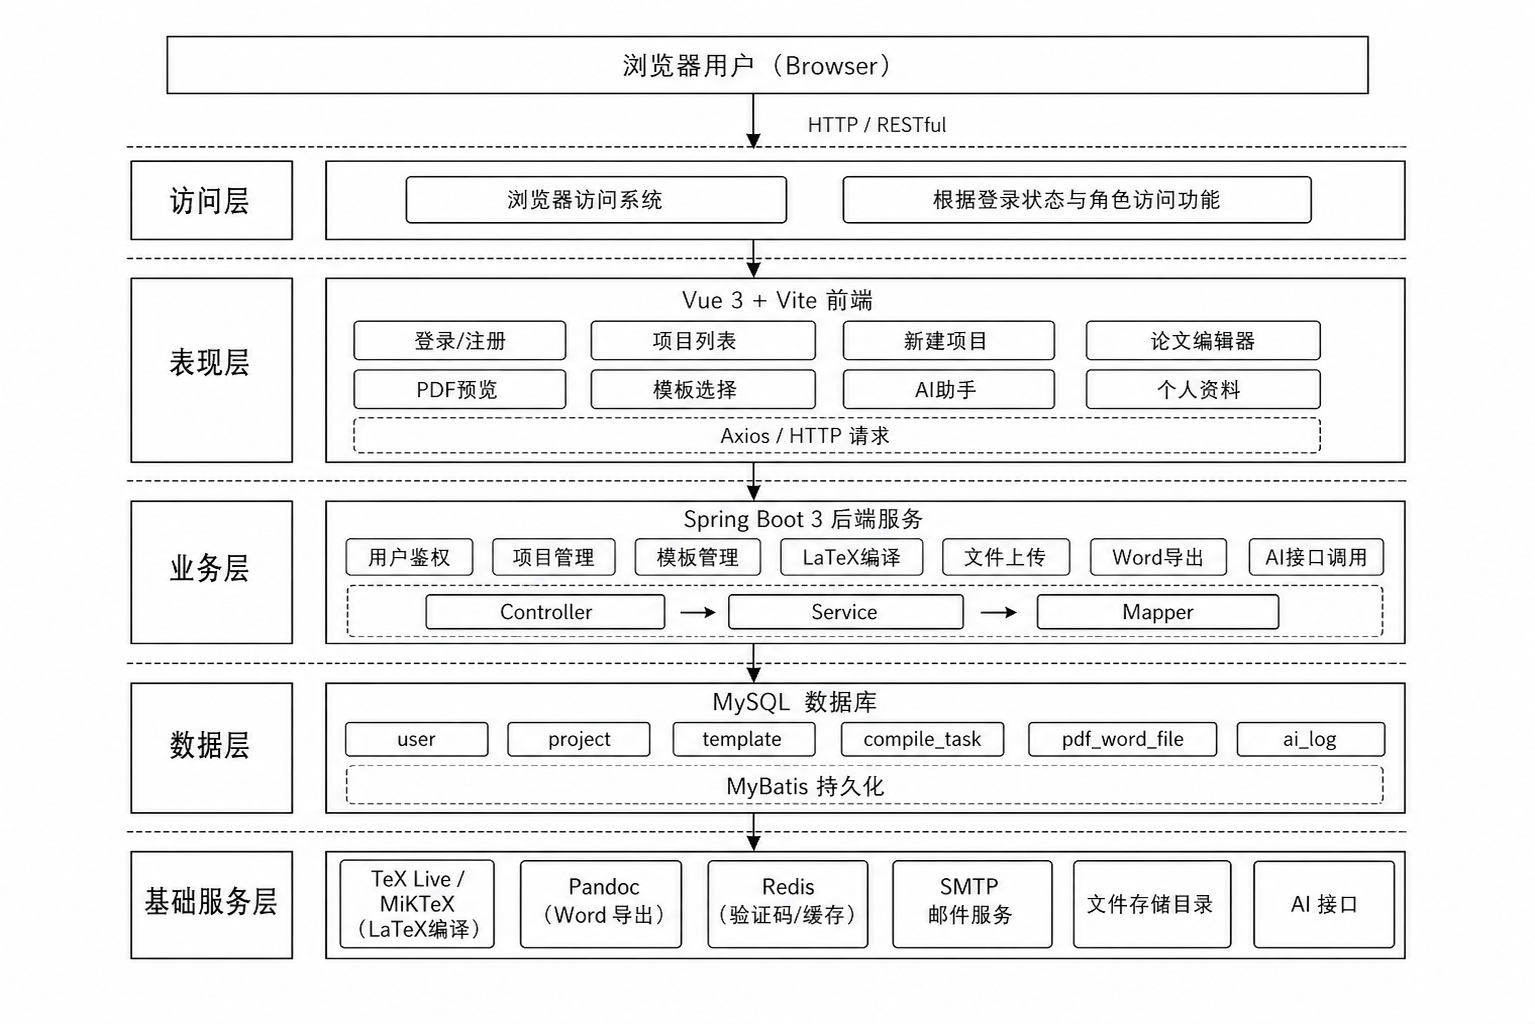
\includegraphics[width=1\linewidth]{ChatGPT Image 2026年4月28日 13_07_15.png}
    \caption{系统总体架构图}
    \label{fig:placeholder}
\end{figure}

\section{功能设计}
根据第三章需求分析结果，系统主要划分为用户管理模块、论文项目管理模块、模板管理模块、LaTeX 在线编辑模块、论文编译模块、文件导出模块和 AI 辅助模块。各模块之间既相互独立，又围绕论文项目形成完整业务流程。

（1）用户管理模块。该模块主要负责用户注册、登录、邮箱验证码、个人资料展示和头像上传等功能。用户注册时需要填写邮箱、用户名和密码，系统通过邮箱验证码校验用户邮箱的有效性。用户登录成功后，后端生成 token 并返回给前端，前端在后续请求中携带 token，后端通过拦截器解析 token 获取用户身份。管理员用户在普通用户权限基础上，可以进行模板导入和模板管理操作。

（2）论文项目管理模块。该模块是系统的核心业务模块，主要负责论文项目的创建、查询、修改和删除。用户可以创建空白项目，也可以基于模板创建项目，还可以通过 PDF 导入方式创建项目。项目创建后，系统将项目名称、LaTeX 内容、所属用户和创建时间等信息保存到数据库中。用户进入项目列表页面后，只能查看自己创建的项目，系统通过用户 ID 进行数据隔离。

（3）模板管理模块。该模块用于管理论文模板资源。普通用户可以查看模板列表，并基于模板创建项目。管理员用户可以新增、修改、删除模板，也可以导入完整的 zip 模板包。由于 LaTeX 模板通常包含 .tex、.cls、.sty、.bib、.bst 和图片等依赖文件，因此系统在模板导入时保留模板目录结构，并在编译阶段复制模板依赖目录，保证模板能够正常编译。

（4）LaTeX 在线编辑模块。该模块为用户提供在线论文编辑能力。系统前端集成 CodeMirror 编辑器，用户可以在浏览器中编辑 LaTeX 源码。编辑器页面还提供组件拖拽插入、图片上传、公式插入、编译引擎选择、PDF 预览和 AI 助手等功能。用户修改论文内容后，可以保存到数据库，也可以直接触发编译生成 PDF。

（5）论文编译模块。该模块负责将 LaTeX 源码编译为 PDF 文件。系统支持 pdflatex、xelatex 和 lualatex 三种编译引擎。后端在编译时创建临时目录，处理图片路径和模板依赖文件，然后调用对应编译命令生成 PDF。如果检测到参考文献信息，系统还可以执行 BibTeX 和多轮 LaTeX 编译，以保证引用编号和参考文献结果正确。

（6）文件导出模块。该模块主要负责 PDF、LaTeX 和 Word 文件导出。PDF 文件由 LaTeX 编译生成，LaTeX 文件由项目源码导出，Word 文件通过 Pandoc 等工具转换生成。导出文件信息可以记录到数据库中，便于用户后续下载和系统进行文件管理。

（7）AI 辅助模块。该模块包括 AI 对话辅助、PDF 转 LaTeX 和编译错误分析等功能。用户可以在编辑器页面向 AI 助手提问，获取 LaTeX 语法、论文排版和模板使用方面的帮助。当论文编译失败时，系统可以将编译日志和相关源码片段提交给 AI 接口，由 AI 返回错误原因和修改建议，从而帮助用户提高错误排查效率。

\section{数据库设计}
数据库设计是系统概要设计的重要组成部分。本系统使用 MySQL 数据库存储业务数据，主要包括用户信息、论文项目、模板信息、编译任务、导出文件和 AI 日志等。数据库设计需要保证数据结构清晰、关系明确，并能够满足系统主要业务流程的需要。

\subsection{ER 图}
根据系统业务关系，可以得到以下实体关系：

（1）用户与项目之间是一对多关系。一个用户可以创建多个论文项目，一个论文项目只属于一个用户。

（2）项目与编译任务之间是一对多关系。一个项目可以多次编译，每次编译都会产生一条编译记录。

（3）项目与导出文件之间是一对多关系。一个项目可以导出多个 PDF、Word 或 LaTeX 文件。

（4）项目与 AI 日志之间是一对多关系。一个项目可以产生多次 AI 对话或错误分析记录。

（5）模板与项目之间为逻辑关联关系。用户可以基于模板创建项目，但项目创建后主要保存 LaTeX 内容，不强制依赖模板表外键。

\begin{figure}[H]
    \centering
    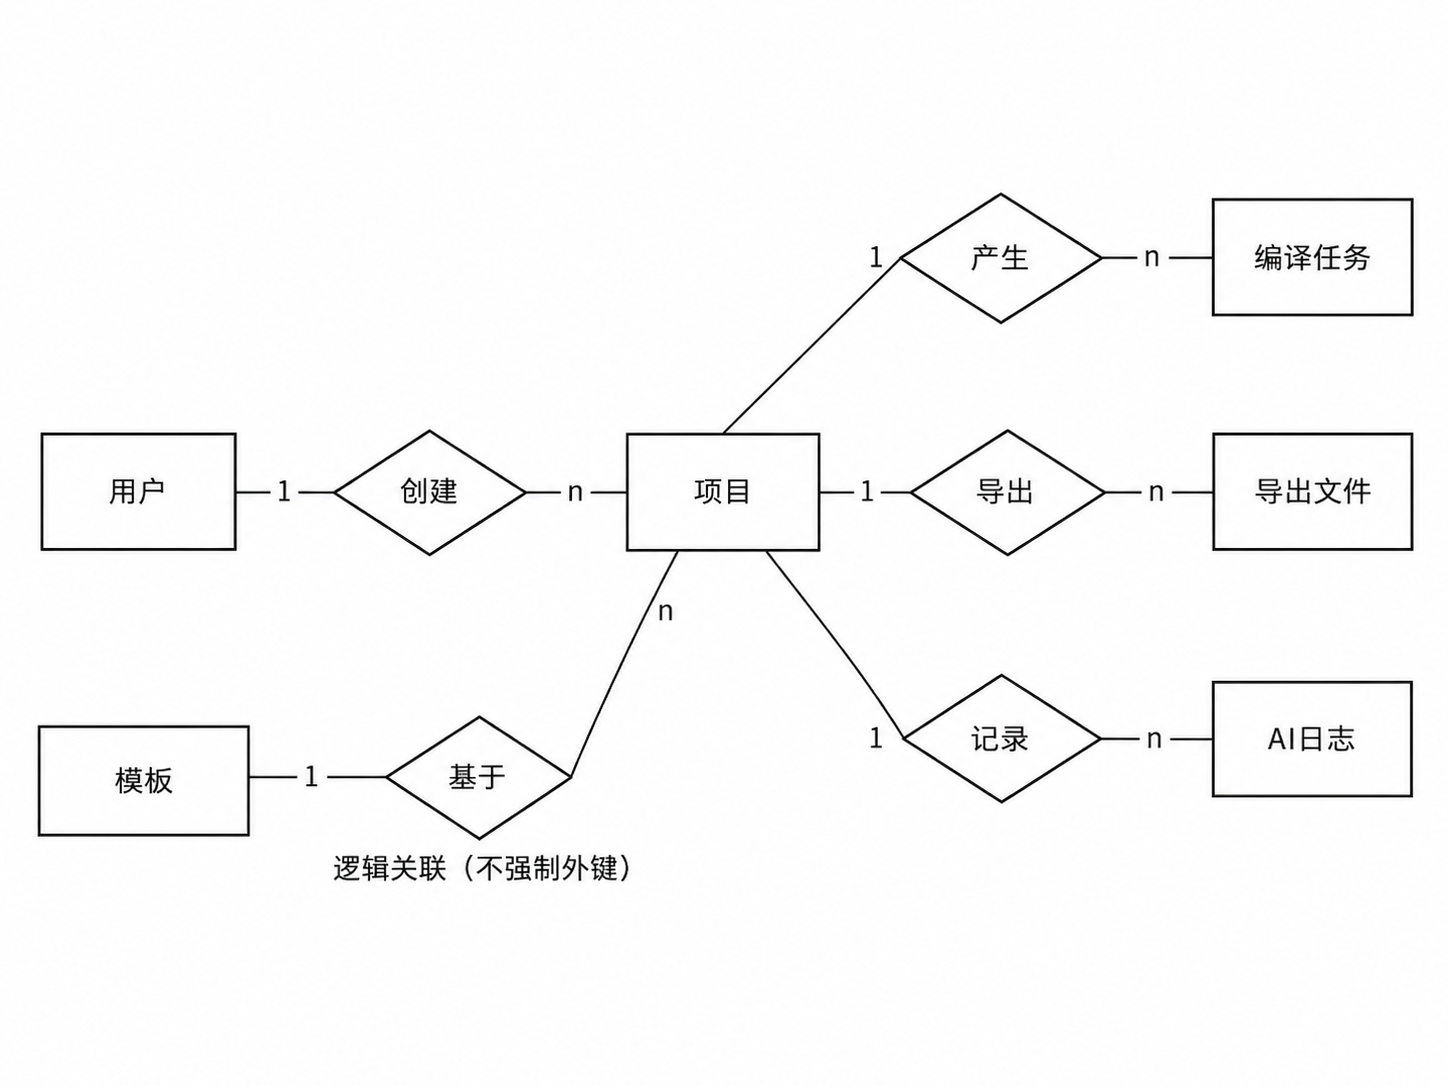
\includegraphics[width=1\linewidth]{ChatGPT Image 2026年4月28日 13_25_16.png}
    \caption{ER 图}
    \label{fig:placeholder}
\end{figure}

\subsection{主要表设计}
本系统主要数据表包括 user、project、template、compile\_task、pdf\_word\_file 和 ai\_log。各表设计如下。 

\begin{table}[H]
    \centering
    \caption{用户表 \texttt{user}}
    \label{tab:user}
    \begin{tabular}{|c|c|c|}
        \hline
        \textbf{字段名} & \textbf{类型} & \textbf{说明} \\ \hline
        \texttt{user\_id} & \texttt{bigint} & 用户 ID，主键 \\ \hline
        \texttt{username} & \texttt{varchar} & 用户名 \\ \hline
        \texttt{email} & \texttt{varchar} & 邮箱 \\ \hline
        \texttt{password\_hash} & \texttt{varchar} & 密码哈希 \\ \hline
        \texttt{avatar\_url} & \texttt{varchar} & 头像地址 \\ \hline
        \texttt{role} & \texttt{varchar} & 用户角色 \\ \hline
    \end{tabular}
\end{table}

用户表用于保存系统用户基本信息。其中 password\_hash 字段用于保存加密后的密码，role 字段用于区分普通用户和管理员。

\begin{table}[H]
    \centering
    \caption{项目表 \texttt{project}}
    \label{tab:project}
    \begin{tabular}{|c|c|c|}
        \hline
        \textbf{字段名} & \textbf{类型} & \textbf{说明} \\ \hline
        \texttt{project\_id} & \texttt{bigint} & 项目 ID，主键 \\ \hline
        \texttt{name} & \texttt{varchar} & 项目名称 \\ \hline
        \texttt{latex\_content} & \texttt{text} & \LaTeX{} 源码内容 \\ \hline
        \texttt{user\_id} & \texttt{bigint} & 所属用户 ID \\ \hline
        \texttt{created\_at} & \texttt{datetime} & 创建时间 \\ \hline
        \texttt{updated\_at} & \texttt{datetime} & 更新时间 \\ \hline
    \end{tabular}
\end{table}

项目表是系统核心业务表，用于保存用户论文项目内容。论文编辑、编译、导出等功能均以 project 表中的 LaTeX 内容为基础。

\begin{table}[H]
    \centering
    \caption{模板表 \texttt{template}}
    \label{tab:template}
    \begin{tabular}{|c|c|c|}
        \hline
        \textbf{字段名} & \textbf{类型} & \textbf{说明} \\ \hline
        \texttt{template\_id} & \texttt{bigint} & 模板 ID，主键 \\ \hline
        \texttt{name} & \texttt{varchar} & 模板名称 \\ \hline
        \texttt{description} & \texttt{varchar} & 模板描述 \\ \hline
        \texttt{template\_path} & \texttt{varchar} & 模板文件路径 \\ \hline
        \texttt{preview\_url} & \texttt{varchar} & 模板预览地址 \\ \hline
        \texttt{created\_at} & \texttt{datetime} & 创建时间 \\ \hline
    \end{tabular}
\end{table}

模板表用于保存论文模板信息。管理员导入 zip 模板包后，系统将模板文件保存到服务器目录，并将模板路径记录到数据库中。

\begin{table}[H]
    \centering
    \caption{编译任务表 \texttt{compile\_task}}
    \label{tab:compile-task}
    \begin{tabular}{|c|c|c|}
        \hline
        \textbf{字段名} & \textbf{类型} & \textbf{说明} \\ \hline
        \texttt{task\_id} & \texttt{bigint} & 编译任务 ID \\ \hline
        \texttt{project\_id} & \texttt{bigint} & 项目 ID \\ \hline
        \texttt{engine} & \texttt{varchar} & 编译引擎 \\ \hline
        \texttt{status} & \texttt{varchar} & 编译状态 \\ \hline
        \texttt{log} & \texttt{text} & 编译日志 \\ \hline
        \texttt{result\_pdf\_path} & \texttt{varchar} & PDF 文件路径 \\ \hline
        \texttt{created\_at} & \texttt{datetime} & 创建时间 \\ \hline
        \texttt{completed\_at} & \texttt{datetime} & 完成时间 \\ \hline
    \end{tabular}
\end{table}

编译任务表用于记录项目每次编译结果。系统可以通过该表查询最近一次编译状态，并在编译失败时获取错误日志。

\begin{table}[H]
    \centering
    \caption{导出文件表 \texttt{pdf\_word\_file}}
    \label{tab:pdf-word-file}
    \begin{tabular}{|c|c|c|}
        \hline
        \textbf{字段名} & \textbf{类型} & \textbf{说明} \\ \hline
        \texttt{pdf\_id} & \texttt{bigint} & 文件记录 ID \\ \hline
        \texttt{project\_id} & \texttt{bigint} & 项目 ID \\ \hline
        \texttt{filename} & \texttt{varchar} & 文件名称 \\ \hline
        \texttt{file\_path} & \texttt{varchar} & 文件路径 \\ \hline
        \texttt{uploaded\_at} & \texttt{datetime} & 创建时间 \\ \hline
    \end{tabular}
\end{table}

该表用于记录系统生成的 PDF、Word 等导出文件，便于用户下载和系统管理历史文件。

\begin{table}[H]
    \centering
    \caption{AI 日志表 \texttt{ai\_log}}
    \label{tab:ai-log}
    \begin{tabular}{|c|c|c|}
        \hline
        \textbf{字段名} & \textbf{类型} & \textbf{说明} \\ \hline
        \texttt{id} & \texttt{bigint} & 日志 ID \\ \hline
        \texttt{project\_id} & \texttt{bigint} & 项目 ID \\ \hline
        \texttt{request\_type} & \texttt{varchar} & 请求类型 \\ \hline
        \texttt{input\_content} & \texttt{text} & 输入内容 \\ \hline
        \texttt{output\_content} & \texttt{text} & 输出内容 \\ \hline
        \texttt{created\_at} & \texttt{datetime} & 创建时间 \\ \hline
    \end{tabular}
\end{table}

AI 日志表用于记录 AI 对话和编译错误分析过程，便于后续问题追踪和功能优化。

\section{界面设计}
界面设计直接影响用户使用体验。本系统主要面向不一定熟悉 LaTeX 的普通用户，因此界面设计应尽量简洁、清晰，使用户能够快速完成论文创建、编辑、编译和导出操作。系统主要界面包括登录注册页面、项目列表页面、新建项目页面、编辑器页面和个人资料页面。

\subsection{登录注册页面设计}
登录注册页面是用户进入系统的入口。登录页面主要包括账号输入框、密码输入框和登录按钮。注册页面主要包括用户名、邮箱、密码、验证码输入框和发送验证码按钮。用户完成注册后可以使用账号登录系统。登录成功后，系统跳转至项目列表页面。

\begin{figure}[H]
    \centering
    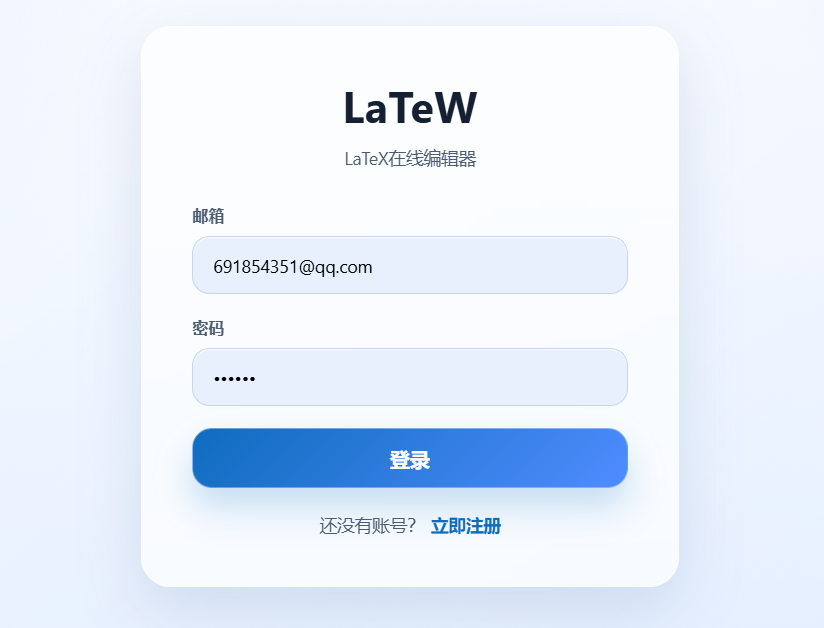
\includegraphics[width=1\linewidth]{QQ20260428-182813.png}
    \caption{登录注册页面设计}
    \label{fig:placeholder}
\end{figure}

\subsection{项目列表与新建项目页面设计}

项目列表页面用于展示当前用户已有论文项目。页面应显示项目名称、更新时间和操作按钮，用户可以进入编辑、删除项目或下载编译结果。管理员用户在该页面可以看到模板导入入口。

\begin{figure}[H]
    \centering
    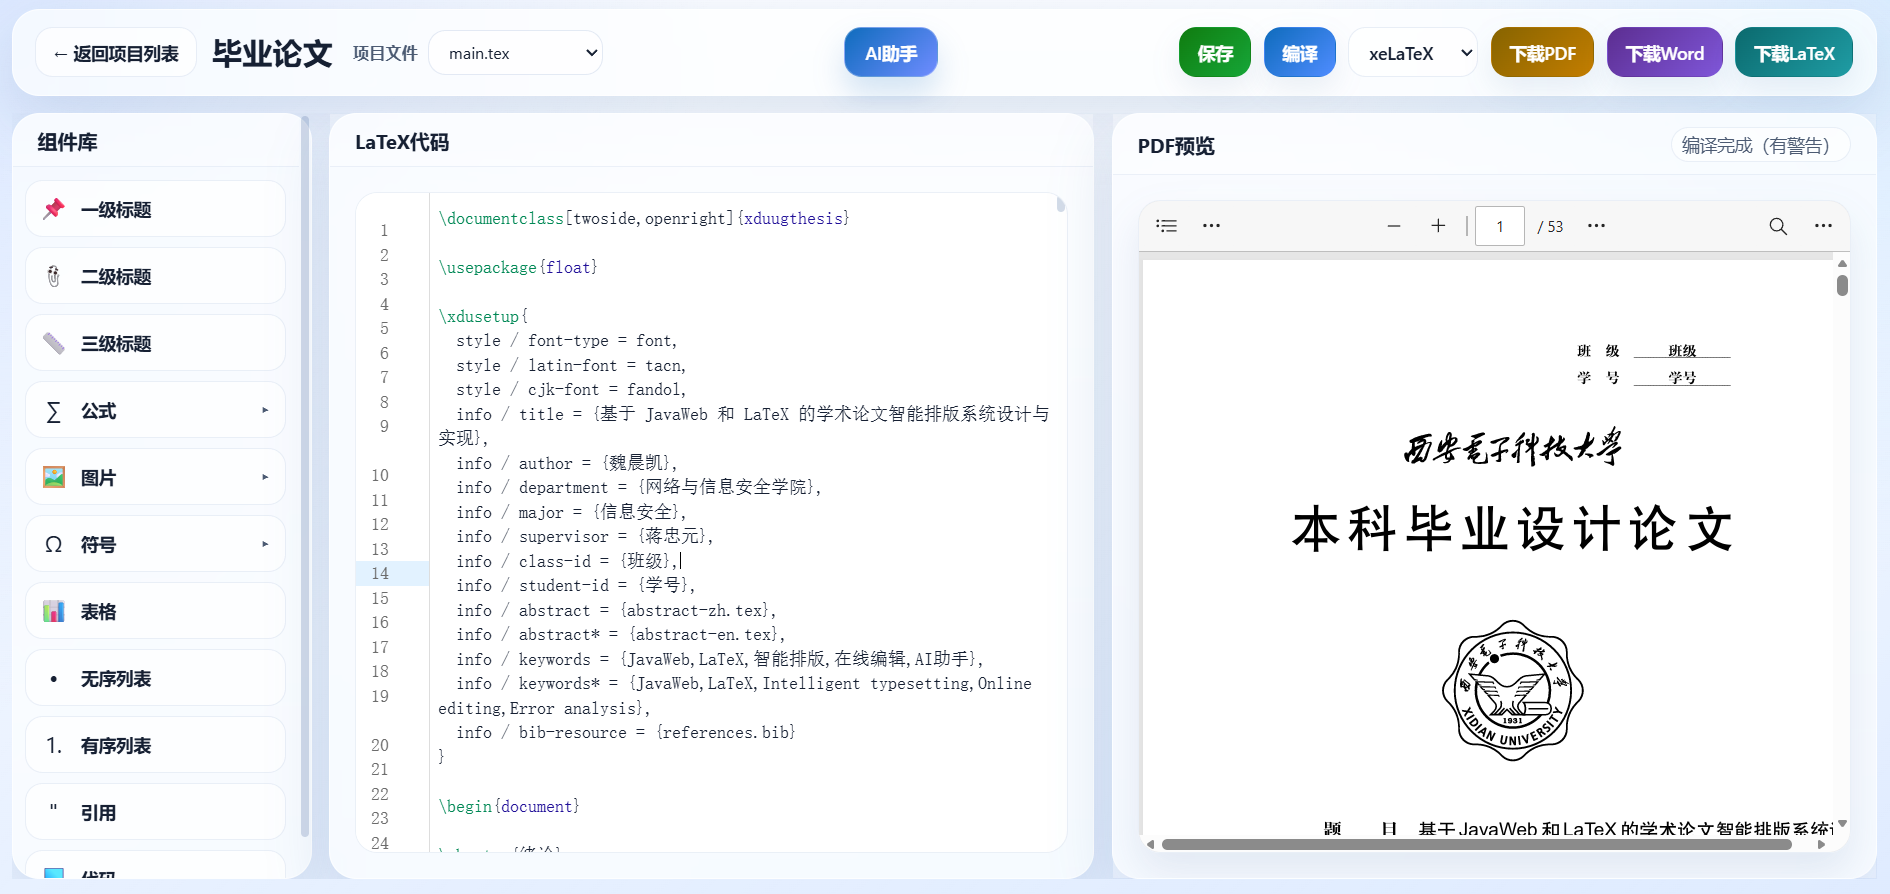
\includegraphics[width=1\linewidth]{image.png}
    \caption{项目列表页面设计}
    \label{fig:placeholder}
\end{figure}

新建项目页面提供三种创建方式：空白创建、模板创建和 PDF 导入创建。空白创建适合用户自行编写论文；模板创建适合用户快速生成论文基本结构；PDF 导入创建则适合用户将已有 PDF 内容转换为 LaTeX 项目。

\begin{figure}[H]
    \centering
    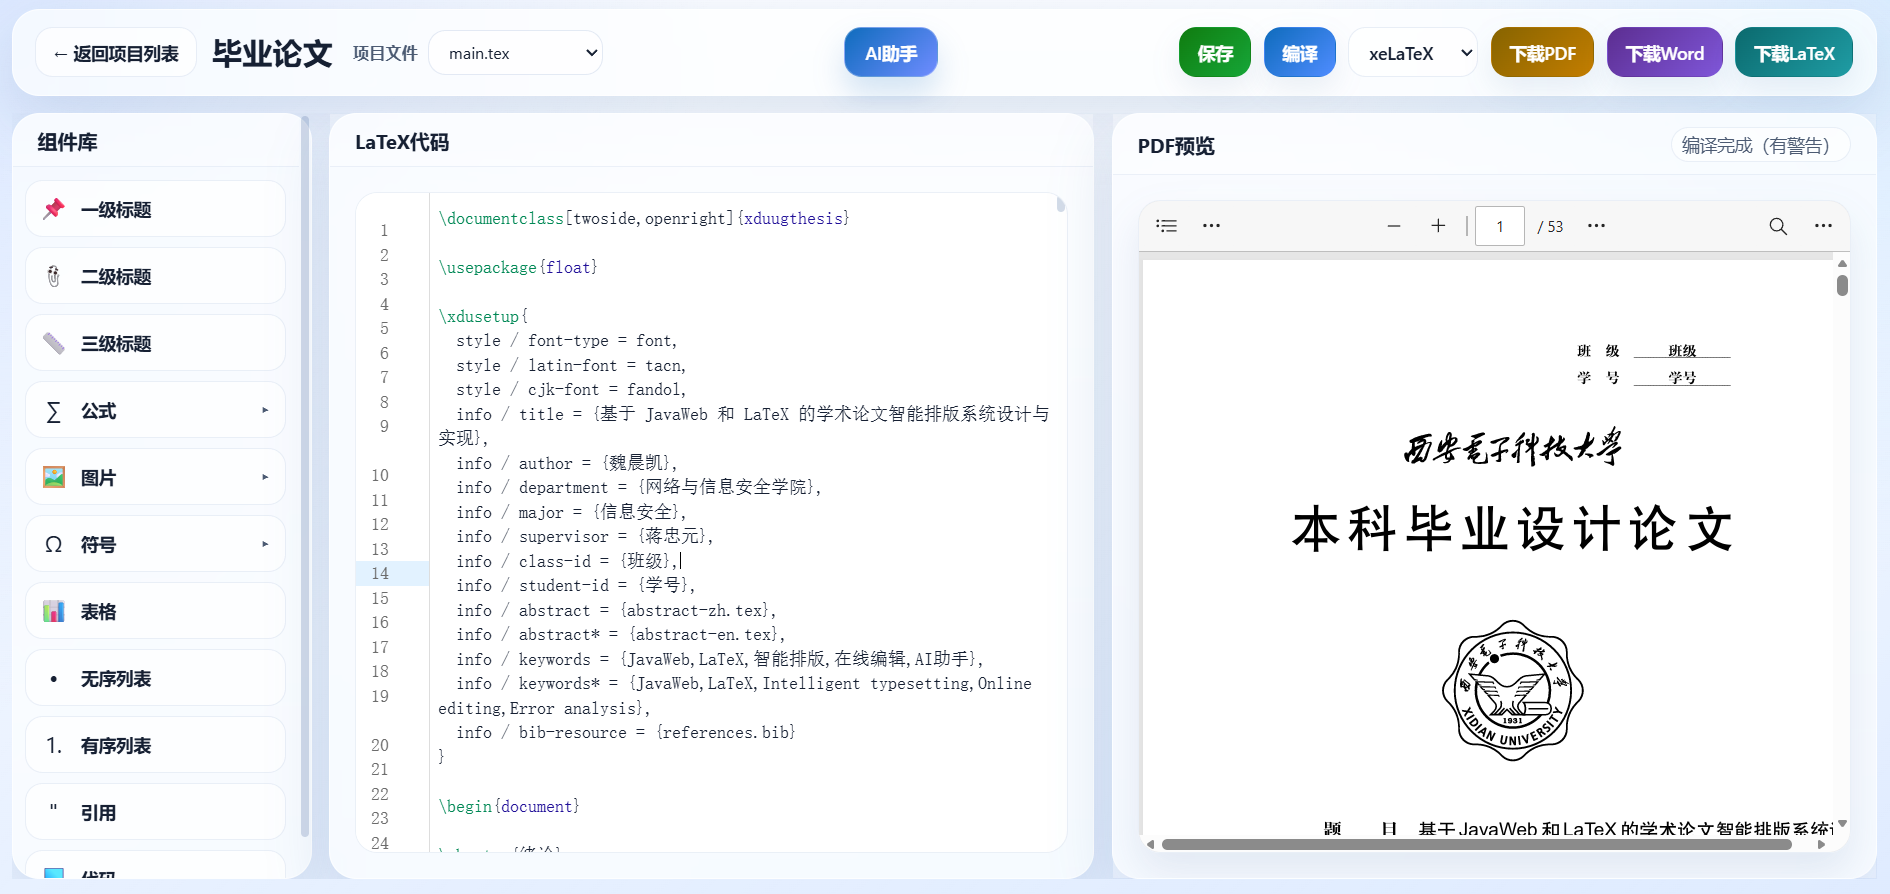
\includegraphics[width=1\linewidth]{image.png}
    \caption{新建项目页面设计}
    \label{fig:placeholder}
\end{figure}

\subsection{编辑器页面设计}
编辑器页面是系统最核心的页面。该页面主要分为三个区域：左侧或上方为工具栏，中间为 LaTeX 源码编辑区，右侧为 PDF 预览区。工具栏提供导入tex文件、保存、编译、选择编译引擎、导出 PDF、导出 Word、导出 LaTeX 等操作。源码编辑区用于编辑 LaTeX 内容，PDF 预览区用于展示编译结果和错误日志。

在编辑器页面中，用户可以完成从论文编辑到编译预览的主要流程。当编译成功时，系统刷新 PDF 预览区域；当编译失败时，系统显示错误日志，并提供 AI 分析入口。这样的界面设计可以减少页面跳转，使论文写作流程更加连贯。

\begin{figure}
    \centering
    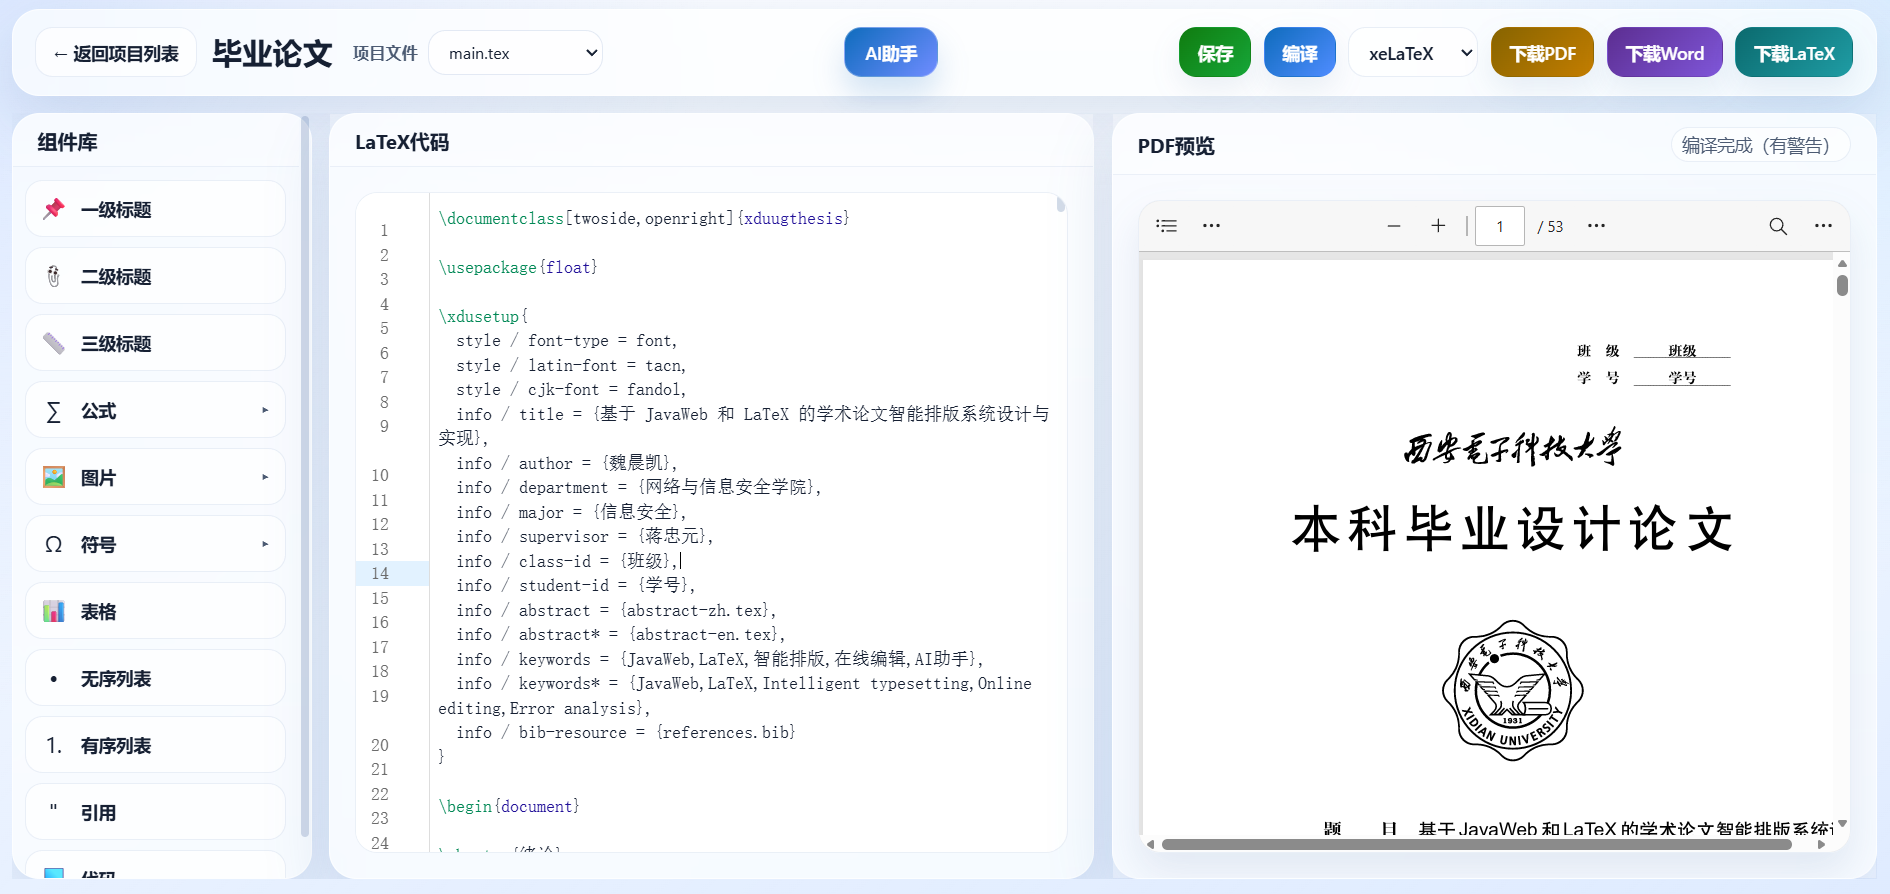
\includegraphics[width=1\linewidth]{image.png}
    \caption{编辑器页面设计}
    \label{fig:placeholder}
\end{figure}

\subsection{个人资料页面设计}
个人资料页面用于展示和修改用户基本信息。页面主要包括头像、用户名、邮箱和用户ID。用户可以上传头像或修改用户名。该页面作为用户管理模块的补充，增强系统的完整性。

\begin{figure}[H]
    \centering
    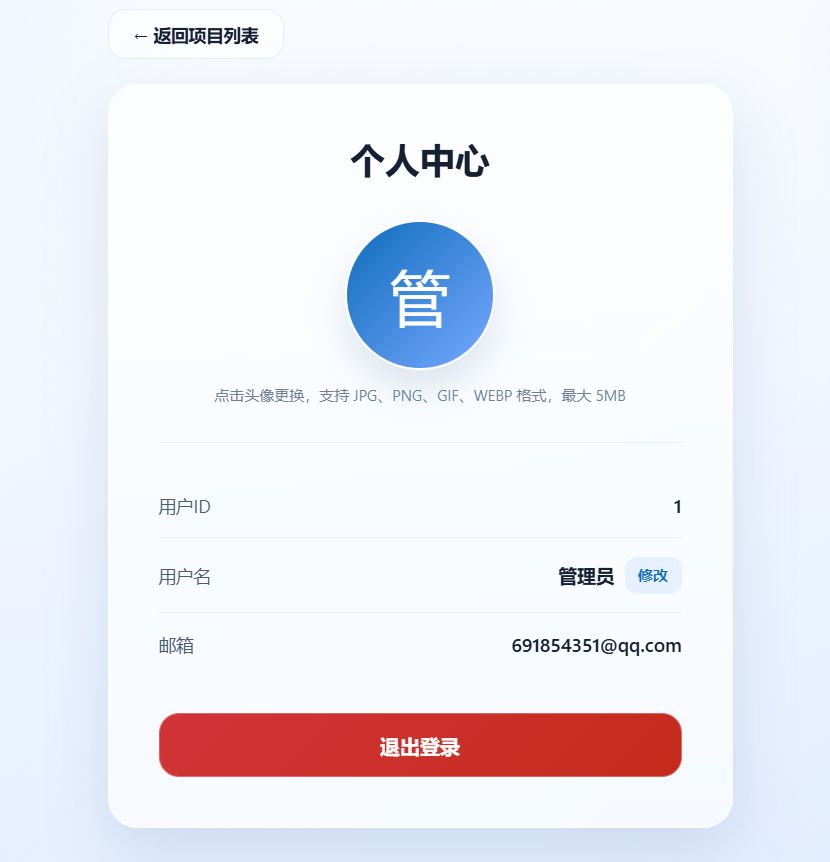
\includegraphics[width=1\linewidth]{QQ20260428-183543.png}
    \caption{个人资料页面设计}
    \label{fig:placeholder}
\end{figure}

\section{本章小结}
本章对基于 JavaWeb 和 LaTeX 的学术论文智能排版系统进行了概要设计。首先介绍了系统总体架构，明确系统采用 B/S 架构和前后端分离模式，并从访问层、表现层、业务层、数据层和基础服务层对系统结构进行了划分。其次，根据需求分析结果，对系统功能模块进行了设计，包括用户管理、论文项目管理、模板管理、LaTeX 在线编辑、论文编译、文件导出和 AI 辅助等模块。然后，对系统数据库进行了概要设计，说明了主要实体关系和核心数据表结构。最后，对系统主要界面进行了设计，包括登录注册页面、项目列表页面、新建项目页面、编辑器页面和个人资料页面。本章内容为下一章系统详细设计与实现提供了基础。

\chapter{系统详细设计与实现}
本章在前文需求分析和概要设计的基础上，对基于 JavaWeb 和 LaTeX 的学术论文智能排版系统进行详细设计与实现说明。系统采用前后端分离架构，前端主要负责用户界面展示和交互操作，后端主要负责业务逻辑处理、数据库访问、文件管理、LaTeX 编译和 AI 接口调用。本章将从开发环境、系统框架、用户管理、论文项目管理、模板管理、LaTeX 在线编辑、论文编译与预览、AI 辅助等方面展开说明。

\section{开发环境}

本系统开发过程中使用的主要软硬件环境如表5.1所示。

\begin{table}[H]
    \centering
    \caption{系统开发环境}
    \label{tab:development-environment}
    \begin{tabular}{|c|c|}
        \hline
        \textbf{环境类型} & \textbf{配置内容} \\ \hline
        操作系统 & Windows 11 \\ \hline
        前端框架 & Vue 3、Vite \\ \hline
        前端编辑器 & Visual Studio Code \\ \hline
        后端框架 & Spring Boot 3 \\ \hline
        后端语言 & Java \\ \hline
        持久层框架 & MyBatis \\ \hline
        数据库 & MySQL \\ \hline
        缓存服务 & Redis \\ \hline
        \LaTeX{} 编译环境 & TeX Live \\ \hline
        文档转换工具 & Pandoc \\ \hline
        主要开发工具 & IntelliJ IDEA、DataGrip、Cursor \\ \hline
        浏览器 & Chrome / Edge \\ \hline
    \end{tabular}
\end{table}

系统前端采用 Vue 3 和 Vite 进行开发，利用组件化方式组织页面结构。后端采用 Spring Boot 3 构建 RESTful 接口，使用 MyBatis 完成数据库访问。数据库采用 MySQL 保存用户、项目、模板、编译任务和 AI 日志等信息。LaTeX 编译功能依赖 TeX Live 环境，Word 导出功能依赖 Pandoc 等文档转换工具。

\section{用户管理模块的设计与实现}
用户管理模块主要实现用户注册、登录、邮箱验证码、个人资料和头像上传等功能。该模块是系统的基础模块，后续项目管理、模板管理、论文编译和 AI 辅助等功能都依赖用户身份信息。

用户注册流程为：用户在注册页面填写用户名、邮箱、密码和验证码，前端提交注册请求，后端首先校验邮箱验证码是否正确，然后判断邮箱或用户名是否已存在。如果校验通过，后端对密码进行加密处理，并将用户信息保存到 user 表中。

用户登录流程为：用户输入账号和密码后，后端根据账号查询用户信息，并对用户输入密码与数据库中保存的加密密码进行匹配。验证通过后，系统生成 token 返回给前端。前端保存 token 后，用户即可访问项目列表、编辑器等页面。

用户管理模块的实现重点如下：

（1）密码加密存储。

系统不直接保存用户明文密码，而是在后端对密码进行加密后存储。这样即使数据库信息泄露，也可以降低用户密码被直接获取的风险。

（2）邮箱验证码校验。

系统通过邮件服务向用户邮箱发送验证码，并将验证码临时保存到 Redis 中，同时设置有效时间。用户注册时，后端校验验证码是否正确和是否过期。

（3）登录状态验证。

用户登录成功后，系统生成 token。后续请求中，前端需要在请求头中携带 token，后端通过拦截器解析 token，获取当前用户 ID，并完成权限校验。

（4）头像上传。

用户可以上传头像文件，后端接收文件后保存到服务器指定目录，并将头像访问路径写入用户表。

\begin{figure}[H]
    \centering
    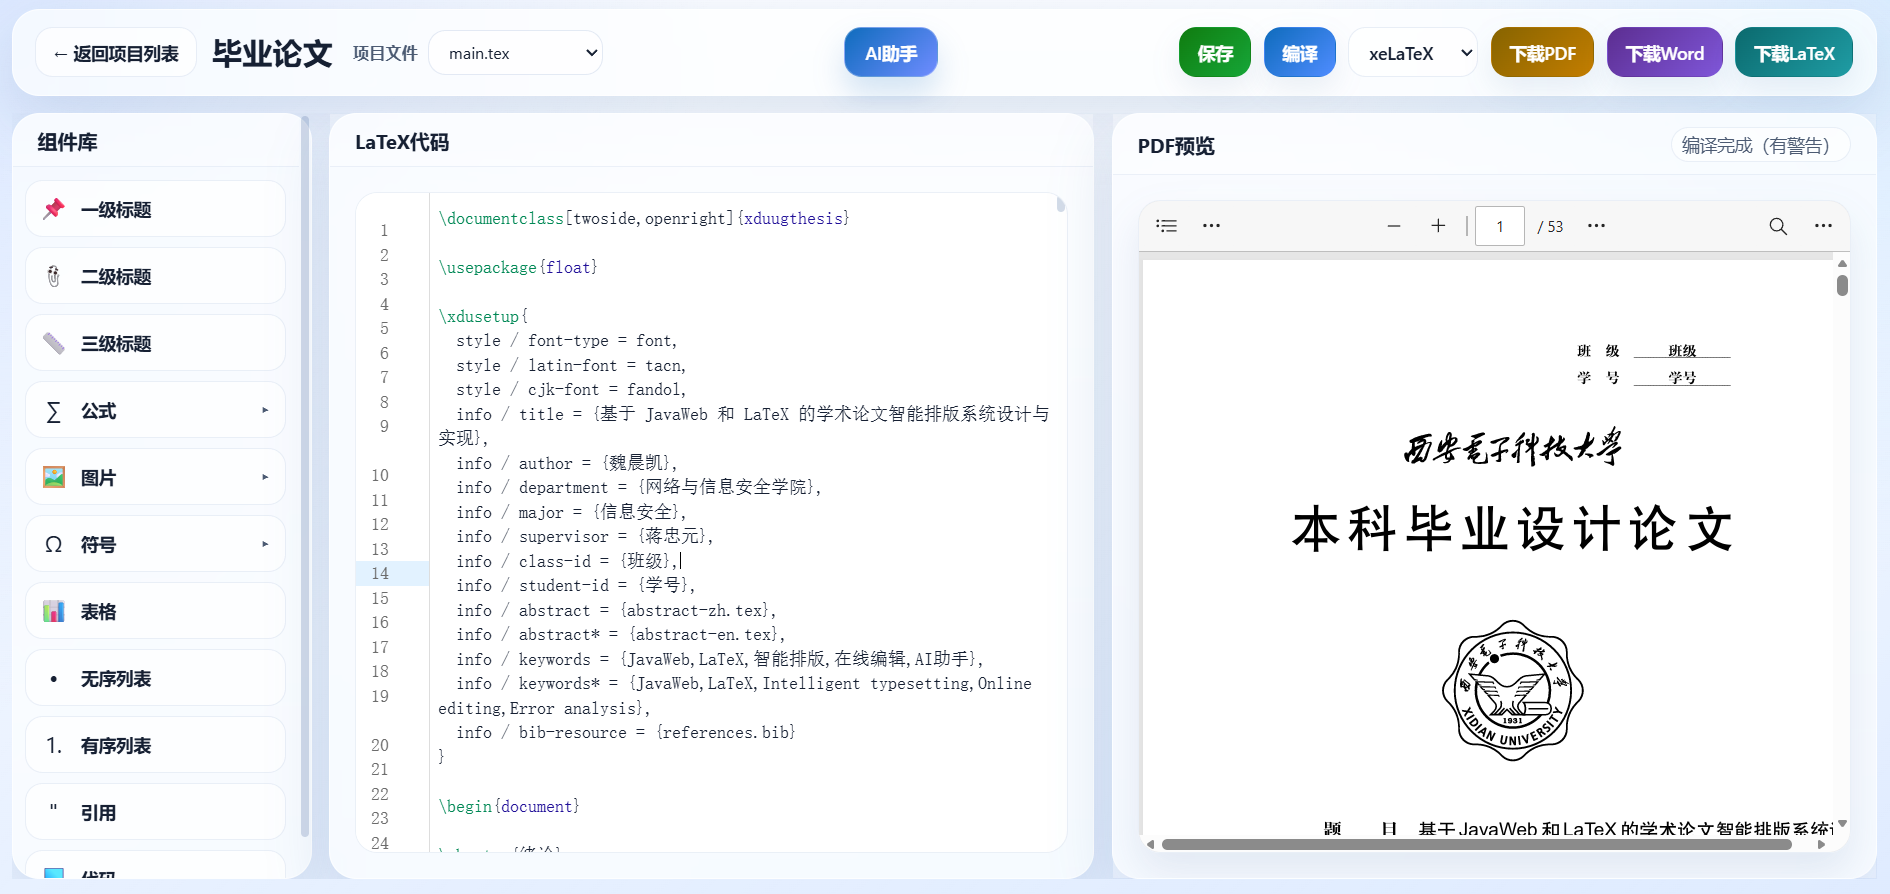
\includegraphics[width=0.75\linewidth]{image.png}
    \caption{登录校验代码片段}
    \label{fig:placeholder}
\end{figure}

\section{论文项目管理模块的设计与实现}
论文项目管理模块是系统的核心模块，用户所有论文内容都以项目为单位进行保存和管理。系统支持空白项目创建、模板项目创建、PDF 导入项目、项目列表查询、项目编辑保存和项目删除等功能。

项目创建时，用户可以选择不同方式。如果用户创建空白项目，系统会生成一个基础 LaTeX 文档结构；如果用户基于模板创建项目，系统会读取模板内容并写入新项目；如果用户通过 PDF 导入创建项目，系统会调用相关解析或 AI 服务，将 PDF 内容转换为 LaTeX 初始内容。

项目保存时，前端将编辑器中的 LaTeX 源码提交给后端，后端根据项目 ID 和当前用户 ID 查询项目是否存在，并判断项目是否属于当前用户。校验通过后，后端更新 project 表中的 latex\_content 和 updated\_at 字段。

项目删除时，系统同样需要进行权限校验，防止用户删除他人的项目。删除操作可以采用物理删除，也可以采用逻辑删除方式。本系统是直接删除项目记录，但在后续扩展中可以增加回收站功能。

\begin{figure}[H]
    \centering
    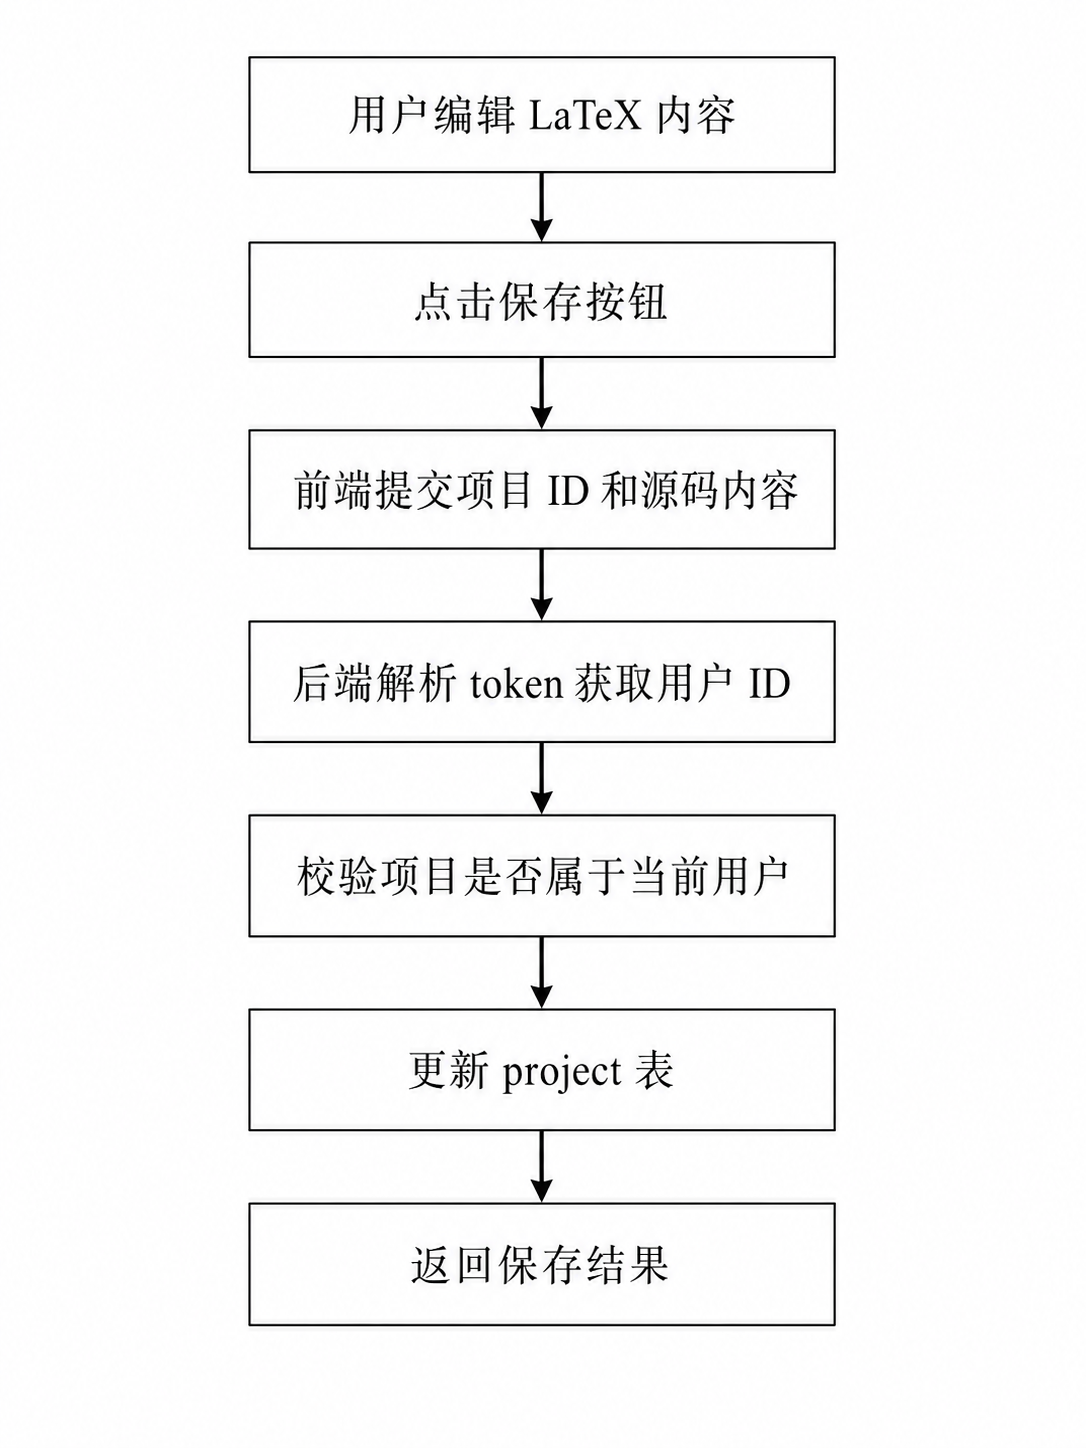
\includegraphics[width=0.75\linewidth]{ChatGPT Image 2026年4月28日 19_29_56.png}
    \caption{项目保存流程图}
    \label{fig:placeholder}
\end{figure}

\begin{figure}[H]
    \centering
    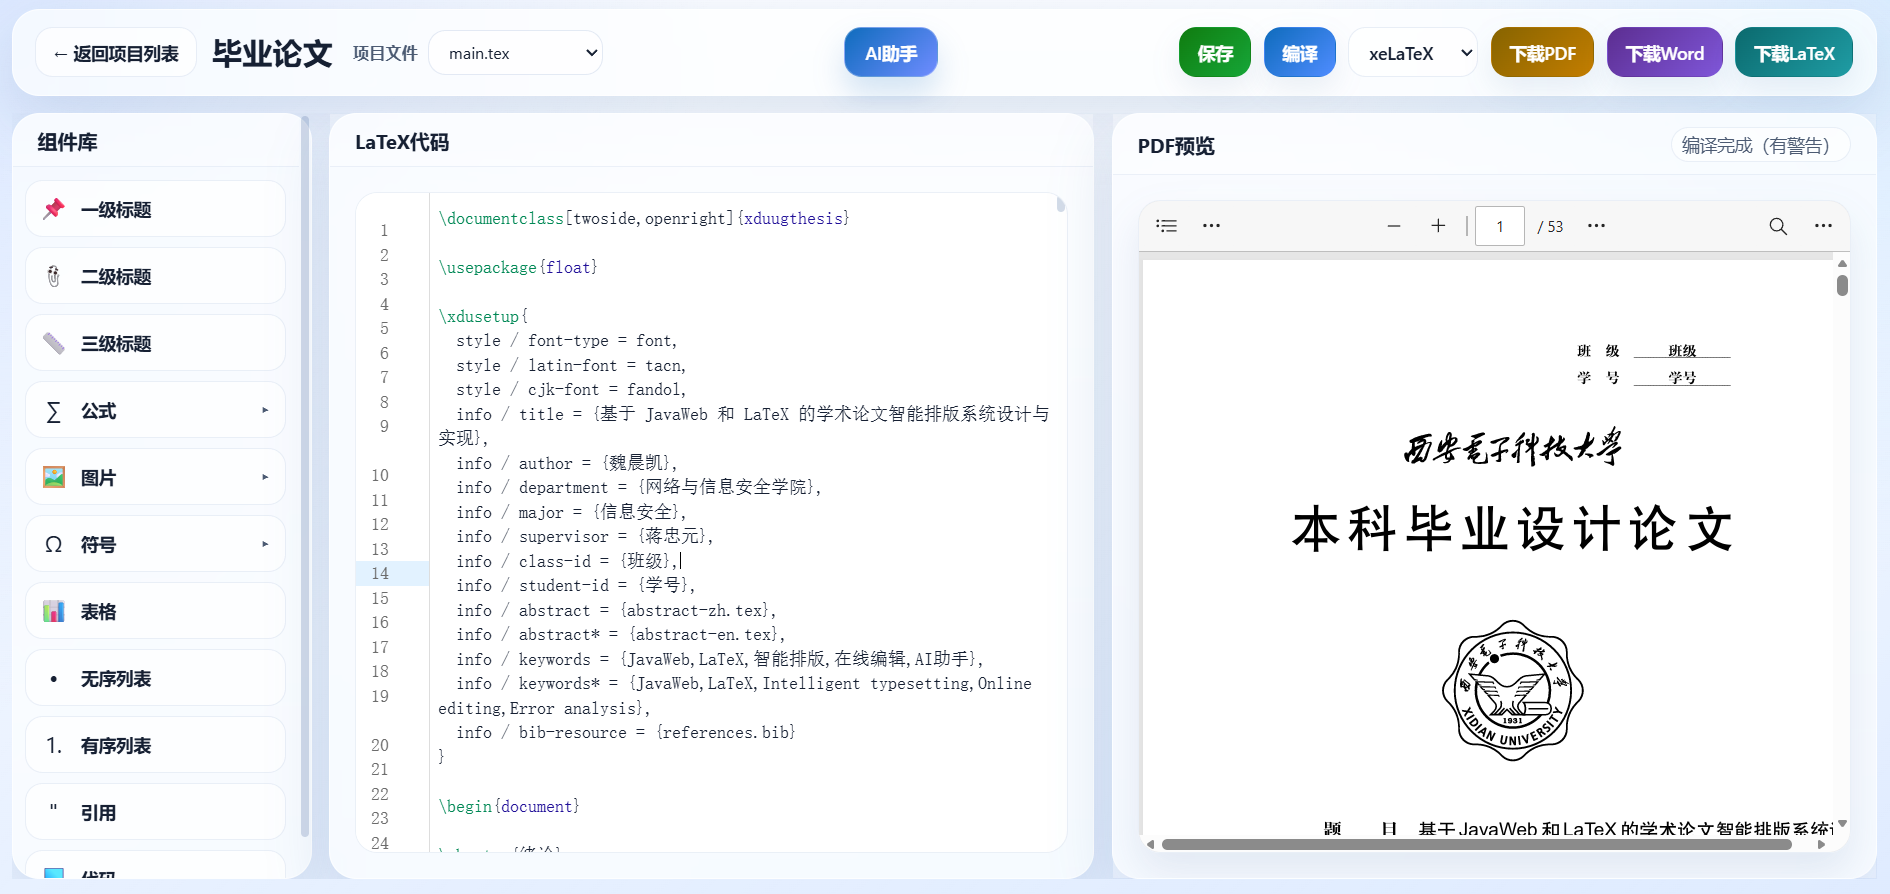
\includegraphics[width=0.75\linewidth]{image.png}
    \caption{更新项目代码片段}
    \label{fig:placeholder}
\end{figure}

\section{模板管理模块的设计与实现}
模板管理模块用于帮助用户快速创建符合格式要求的论文项目。系统模板主要包括模板名称、模板描述、模板文件路径等。普通用户可以查看模板列表并基于模板创建项目，管理员可以新增模板，并上传完整的 zip 模板包。

LaTeX 模板通常不只是一个 .tex 文件，还可能包含 .cls、.sty、.bib、.bst、图片和字体配置等依赖资源。如果系统只保存主 tex 文件，编译时容易出现样式缺失或依赖文件找不到的问题。因此，本系统在模板导入时采用完整 zip 包导入方式，后端解压模板包后保留原始目录结构，并记录模板主文件路径。

模板导入流程为：管理员上传 zip 文件，后端首先校验文件类型，然后解压到模板存储目录。解压完成后，系统扫描目录中的 tex 文件，并选择主 tex 文件作为模板入口。管理员填写模板名称和描述后，系统将模板信息保存到 template 表中。用户基于模板创建项目时，系统读取模板主文件内容，并复制模板依赖目录到项目编译目录中。

模板导入设计的关键在于保留依赖文件。系统在编译基于模板创建的项目时，需要将模板目录中的依赖文件复制到临时编译目录，使 LaTeX 编译器能够找到对应的样式文件、参考文献文件和图片资源。

\begin{figure}[H]
    \centering
    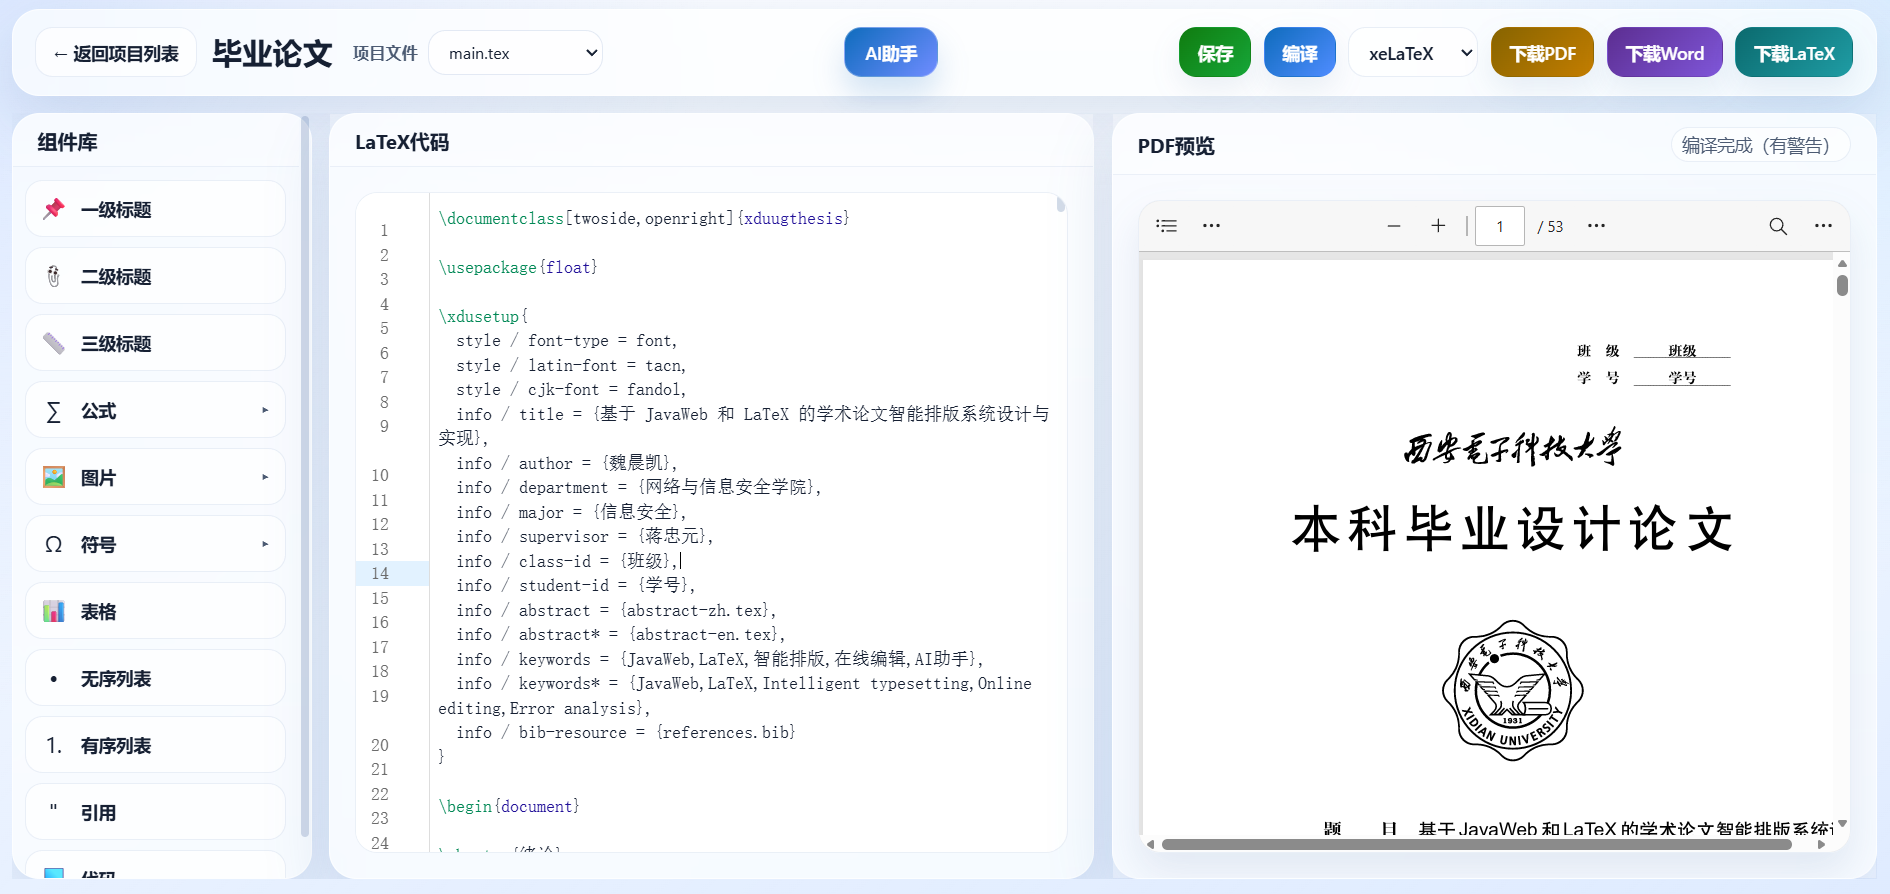
\includegraphics[width=0.75\linewidth]{image.png}
    \caption{模板导入代码片段}
    \label{fig:placeholder}
\end{figure}

\section{LaTeX 在线编辑模块的设计与实现}
LaTeX 在线编辑模块为用户提供浏览器端论文源码编辑功能。系统前端集成 CodeMirror 编辑器，使用户能够获得较好的代码编辑体验。编辑器页面主要包括源码编辑区、PDF 预览区和工具栏区域。

源码编辑区用于显示和修改 LaTeX 内容。用户进入编辑页面后，前端根据项目 ID 请求后端项目详情接口，后端返回项目名称和 LaTeX 内容，前端将内容加载到编辑器中。用户修改内容后，可以点击保存按钮，将当前源码保存到数据库。

工具栏主要提供导入tex文件、保存、编译、导出、AI助手、图片上传、公式插入等操作。用户点击图片上传后，前端提交图片文件给后端，后端保存图片并返回访问路径，前端自动生成 LaTeX 图片插入代码。公式插入功能则通过预设常用公式模板实现。用户选择某个公式后，前端将对应 LaTeX 公式代码插入到光标位置，减少用户手动输入复杂命令的成本。

\begin{figure}[H]
    \centering
    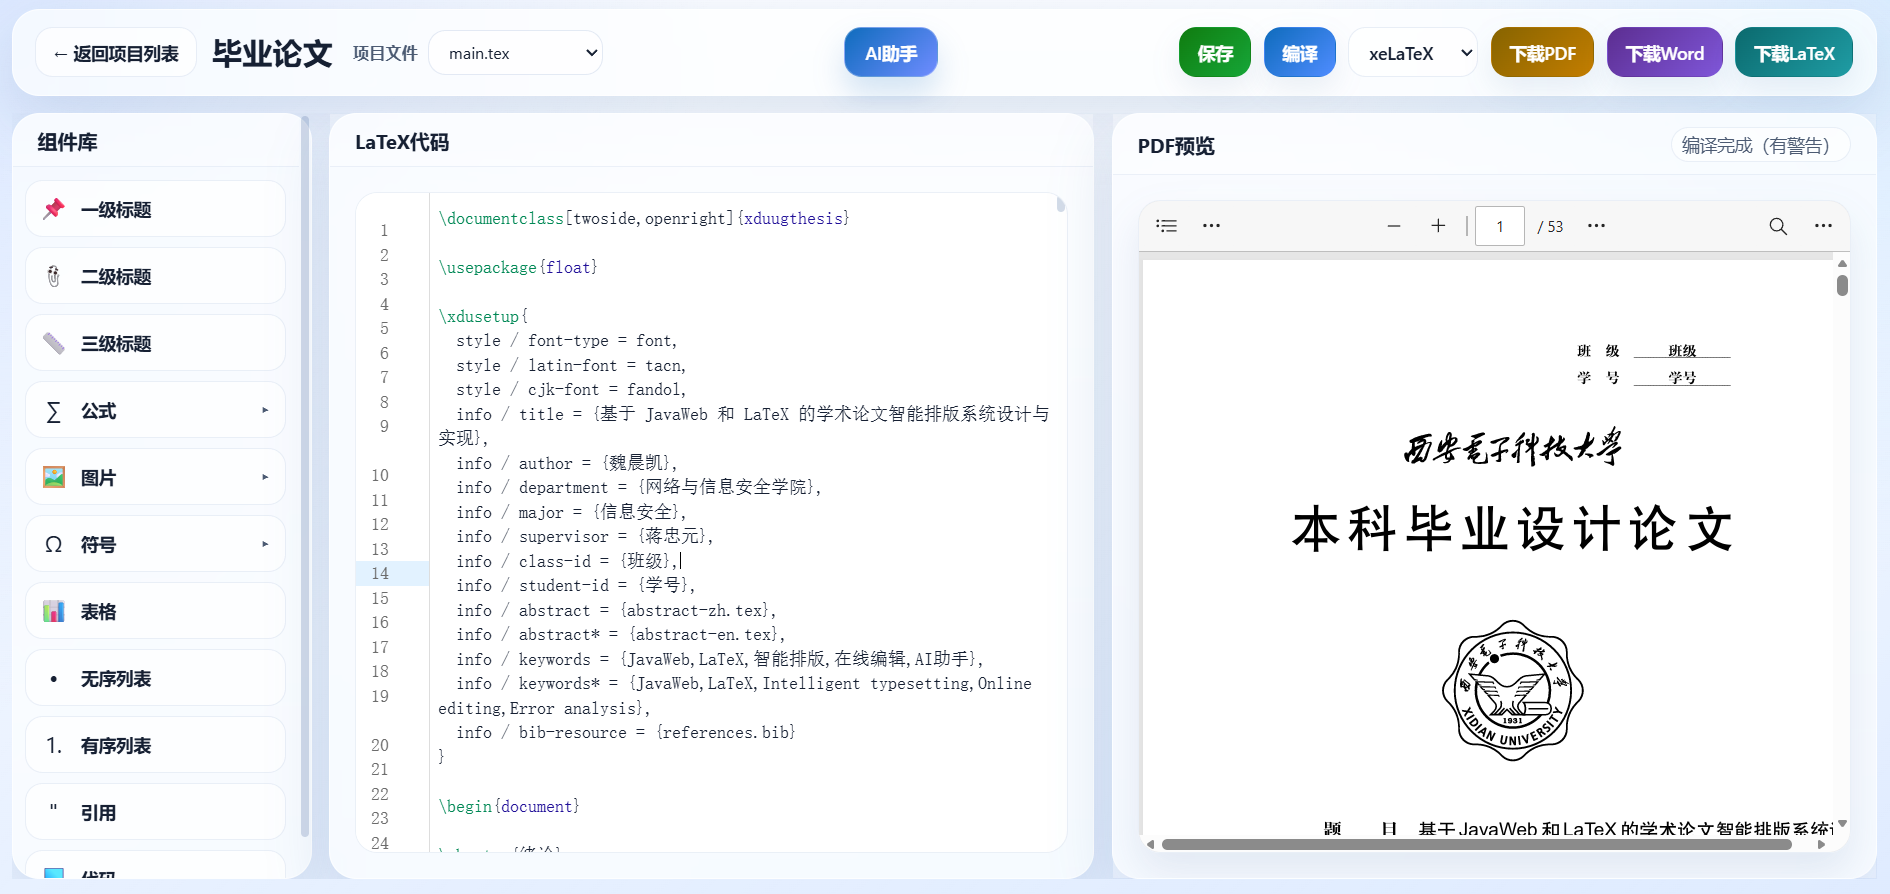
\includegraphics[width=0.75\linewidth]{image.png}
    \caption{在线编辑流程图}
    \label{fig:placeholder}
\end{figure}

\begin{figure}[H]
    \centering
    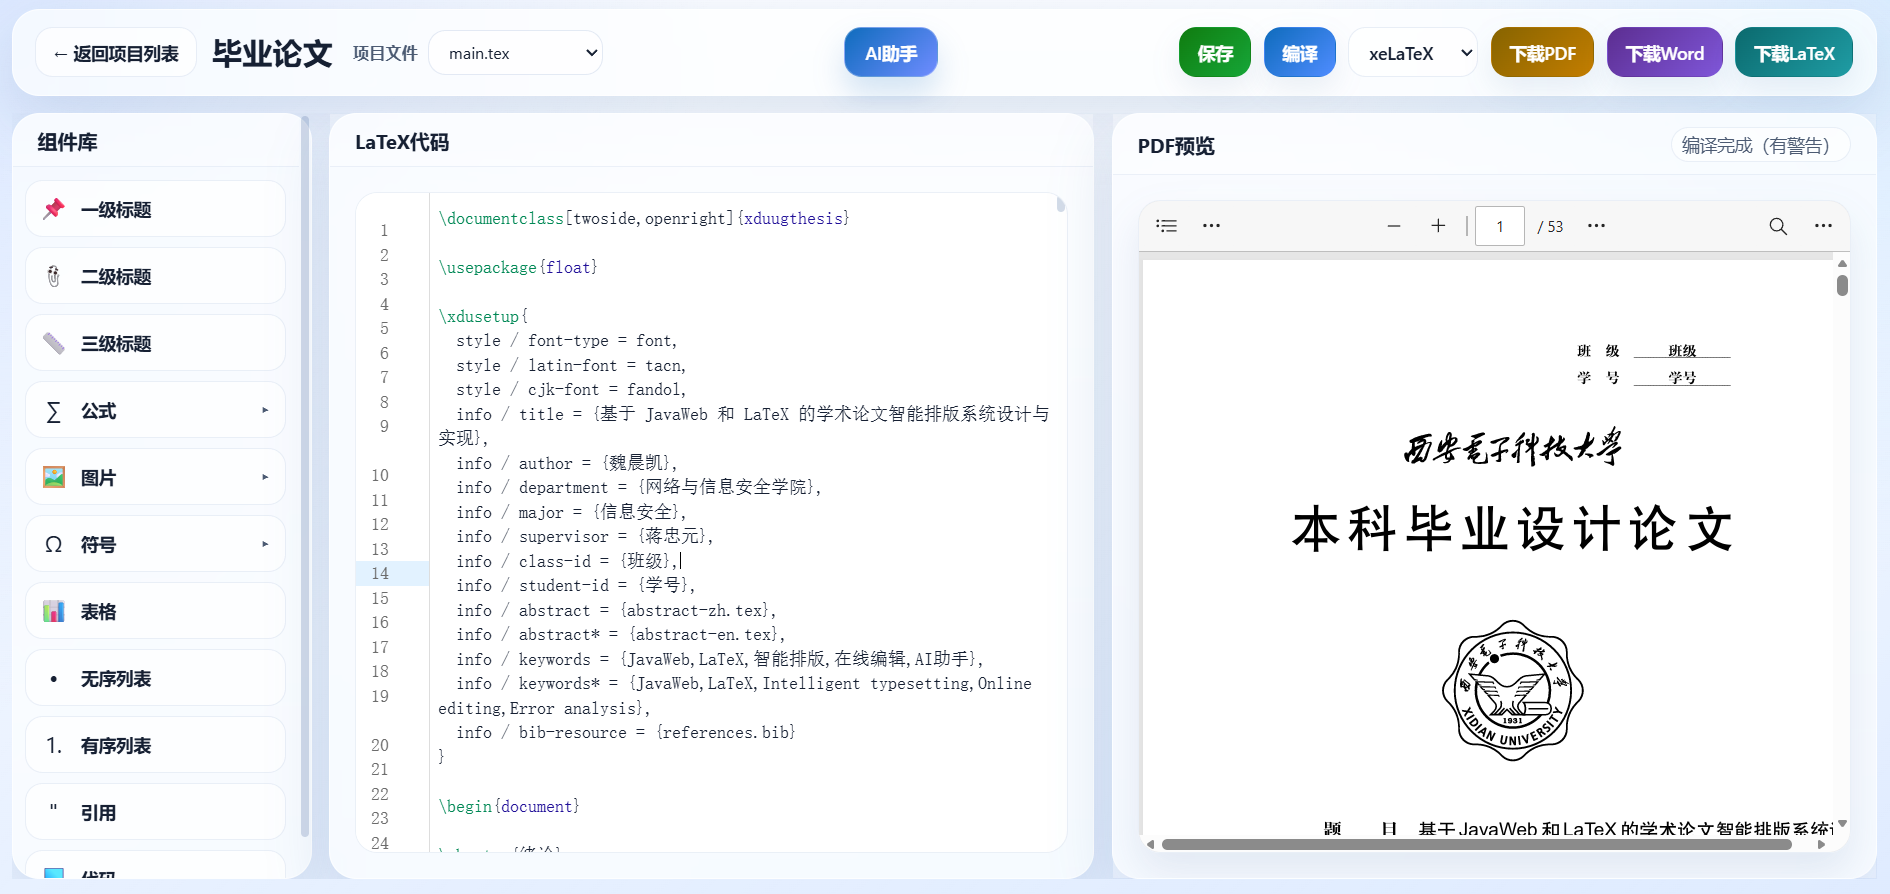
\includegraphics[width=0.75\linewidth]{image.png}
    \caption{拖拽插入代码片段}
    \label{fig:placeholder}
\end{figure}

\section{论文编译与预览模块的设计与实现}
论文编译模块负责将 LaTeX 源码转换为 PDF 文件，是系统最重要的功能之一\cite{wang2012latexaspnet}。用户在编辑器页面点击编译按钮后，前端将项目 ID、LaTeX 内容和编译引擎提交给后端，后端调用本地 LaTeX 编译环境生成 PDF 文件。

系统支持 pdflatex、xelatex 和 lualatex 三种编译引擎。对于中文毕业论文，通常使用 xelatex 更容易处理中文字体问题；对于部分英文期刊模板，pdflatex 兼容性较好；对于需要更强字体控制能力的模板，可以选择 lualatex。

编译实现过程主要包括以下步骤：

（1）创建临时编译目录。

后端为每次编译任务创建独立目录，用于保存 tex 文件、图片资源、模板依赖文件和编译结果，防止不同用户或不同项目之间互相影响。

（2）写入 LaTeX 源码。

系统将用户当前编辑的 LaTeX 内容写入临时目录中的主 tex 文件。

（3）复制模板依赖和图片资源。

如果项目基于模板创建，系统将模板目录中的 .cls、.sty、.bib、.bst 等依赖文件复制到编译目录。若论文中使用了上传图片，也需要保证图片路径能够被编译器识别。

（4）调用编译命令。

后端通过 Java 的 ProcessBuilder 或相关工具调用 LaTeX 编译命令。例如，选择 xelatex 时，系统执行 xelatex 命令生成 PDF 文件。

（5）收集编译日志。

系统读取编译过程输出的日志信息。如果编译成功，则返回 PDF 路径；如果编译失败，则保存错误日志并返回给前端。

（6）返回编译结果。

编译成功后，前端刷新 PDF 预览区域；编译失败后，前端展示错误日志，并提供 AI 分析按钮。

编译任务结果保存到 compile\_task 表中，包括项目 ID、编译引擎、编译状态、日志内容和 PDF 文件路径等信息。这样既可以方便用户查看最近一次编译结果，也可以为 AI 错误分析提供数据来源。

\begin{figure}[H]
    \centering
    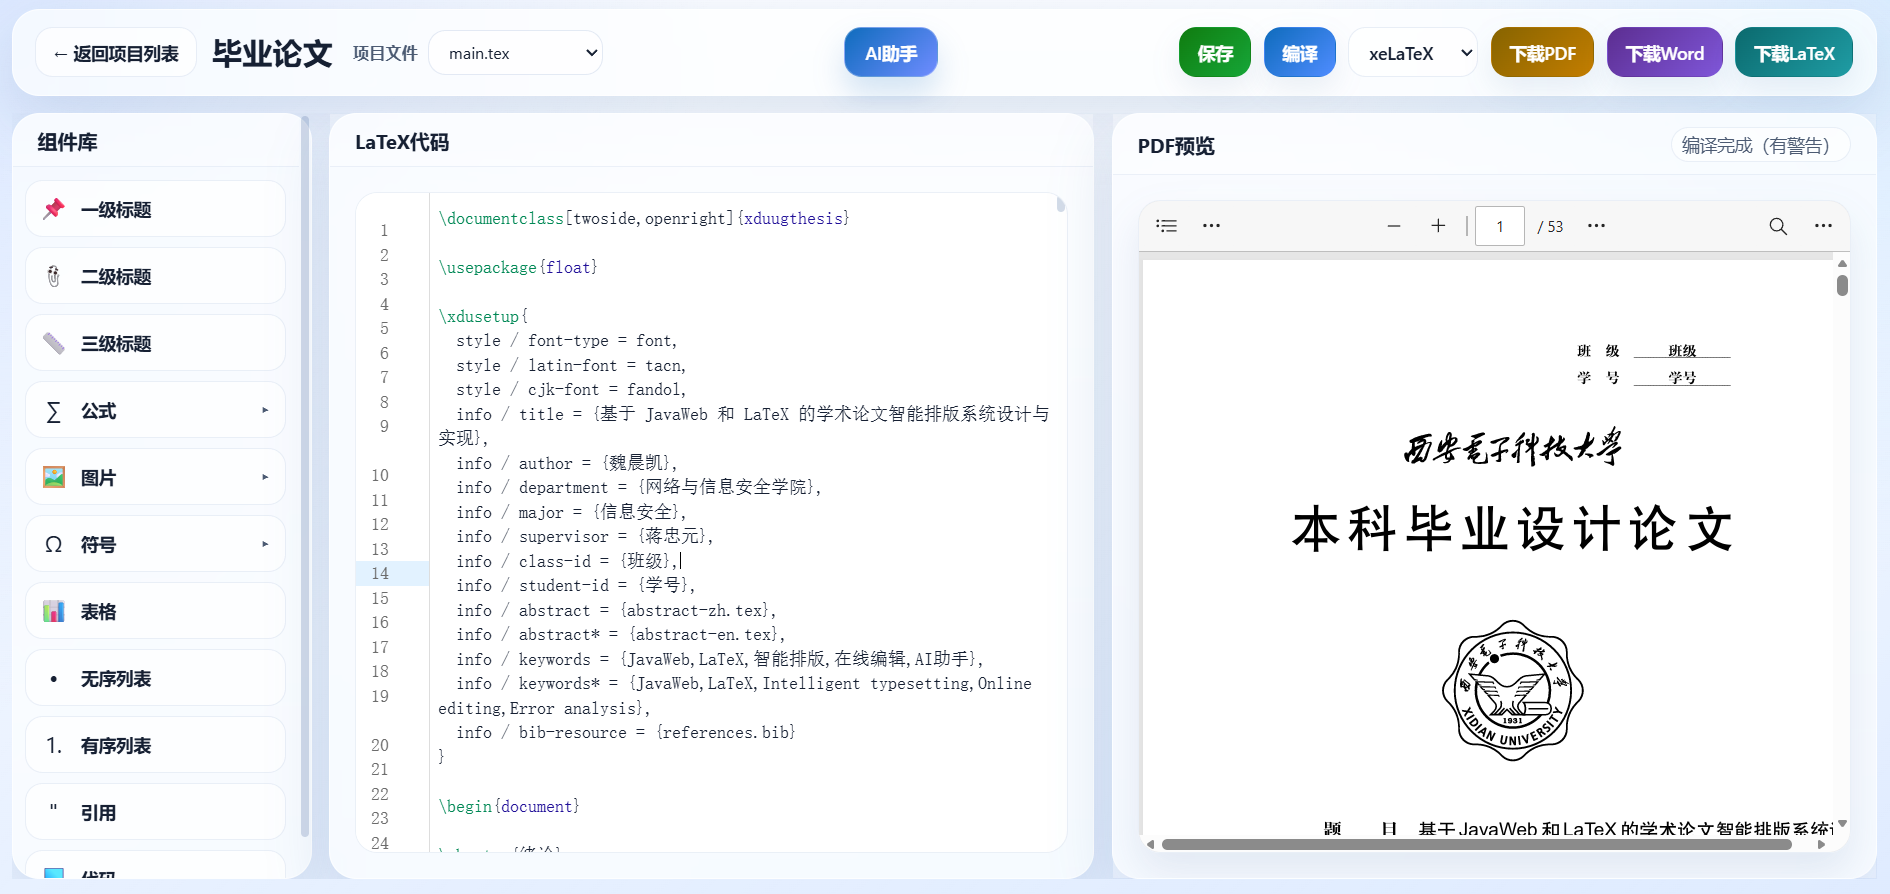
\includegraphics[width=0.75\linewidth]{image.png}
    \caption{论文编译代码片段}
    \label{fig:placeholder}
\end{figure}

\section{文件导出模块的设计与实现}
文件导出模块用于满足用户在不同场景下的论文提交和编辑需求。系统主要支持 PDF、LaTeX 和 Word 三种格式导出。由于不同文档格式在结构表示和排版信息保留方面存在差异，文件转换过程中需要考虑内容结构识别与格式兼容问题\cite{dejean2006pdfxml}。

PDF 导出依赖 LaTeX 编译结果。当论文编译成功后，系统将生成的 PDF 文件保存到指定目录，并提供下载地址。用户点击导出 PDF 时，前端直接请求后端下载接口即可。

LaTeX 导出用于导出项目源码。系统根据项目 ID 查询当前项目的 latex\_content 字段，并生成 .tex 文件返回给用户。该功能适合用户后续在本地或其他 LaTeX 平台继续编辑。
Word 导出则通过文档转换工具实现。后端可以将 LaTeX 源码或编译生成的中间文件交由 Pandoc 转换为 .docx 文件。转换完成后，系统记录文件路径，并向前端返回下载链接。由于 LaTeX 与 Word 的排版机制不同，复杂模板、特殊宏包和部分公式环境在转换过程中可能存在兼容性问题，因此 Word 导出主要满足基础内容转换需求。

\begin{figure}[H]
    \centering
    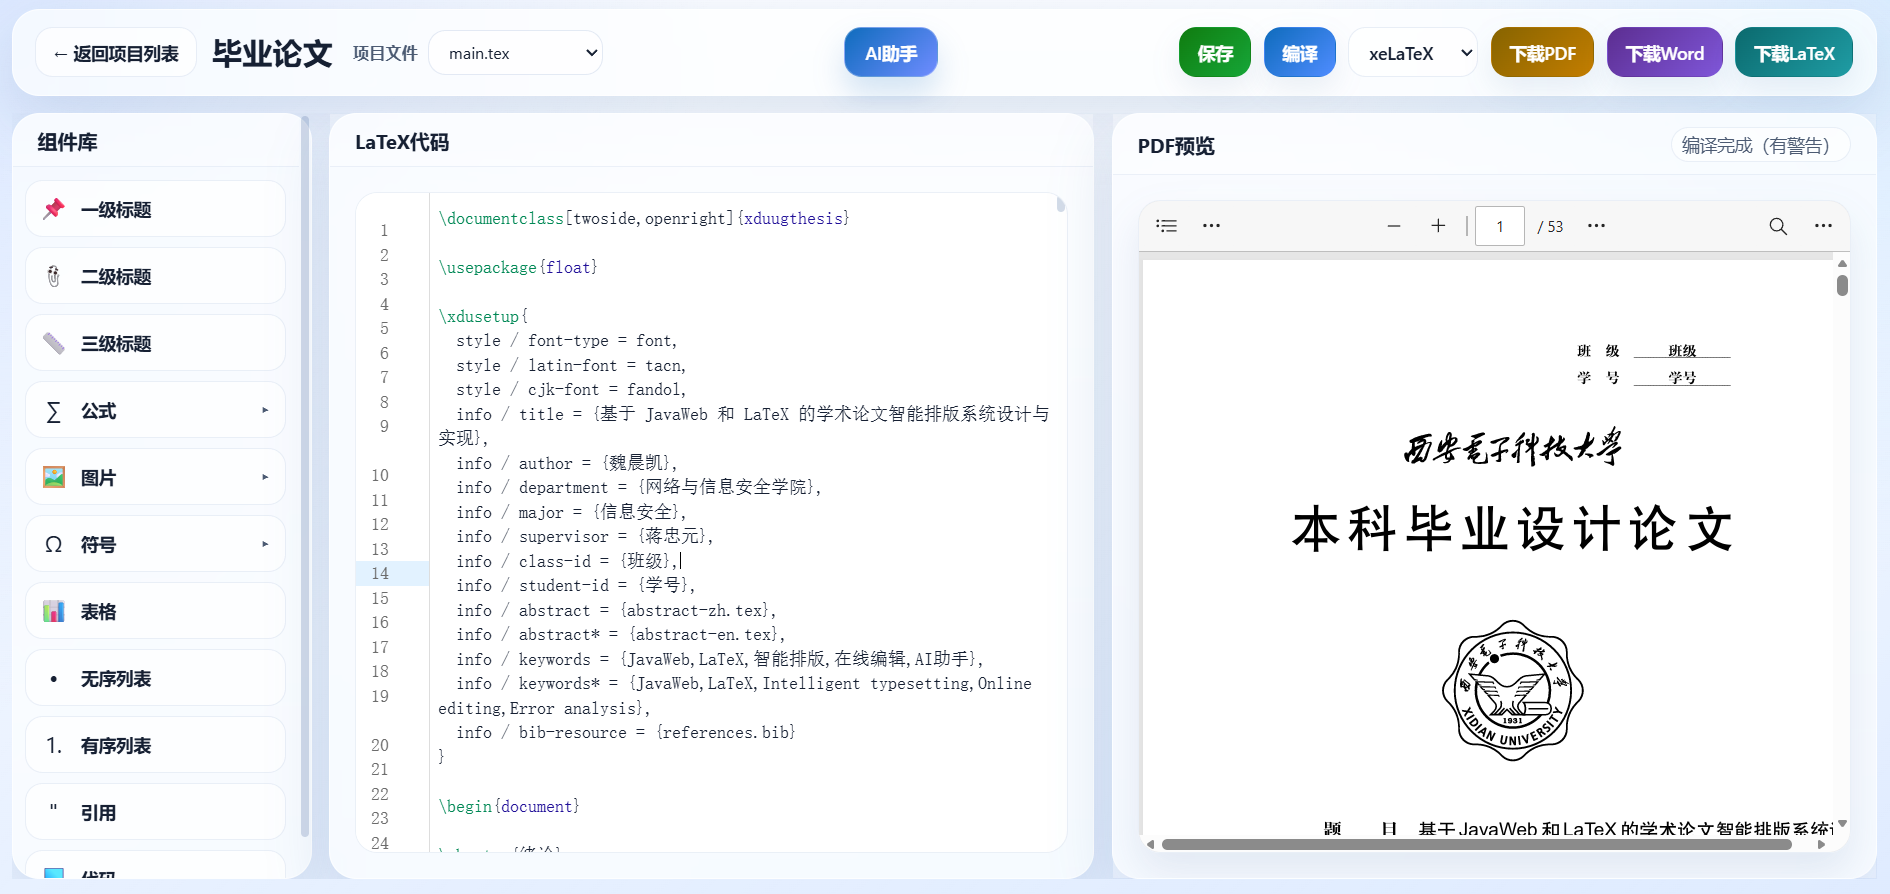
\includegraphics[width=0.75\linewidth]{image.png}
    \caption{pdf下载代码片段}
    \label{fig:placeholder}
\end{figure}

\section{AI 辅助模块的设计与实现}
AI 辅助模块主要包括 AI 对话和编译错误分析两个功能。该模块的目标是降低用户使用 LaTeX 的难度，帮助用户理解排版命令、模板问题和编译错误。

AI 对话功能位于编辑器页面的上方工具栏。用户可以输入问题，例如“如何插入图片”“如何写数学公式”“为什么 xelatex 编译失败”等。前端将用户问题提交给后端，后端封装请求并调用 AI 接口。AI 返回结果后，前端以对话形式展示给用户。

编译错误分析功能与论文编译模块联动。当编译失败时，系统会保存错误日志。用户点击“AI 分析错误”按钮后，后端读取最近一次编译日志，并结合部分 LaTeX 源码构造提示词，请求 AI 分析错误原因。AI 返回内容通常包括错误原因、可能位置和修改建议。前端将分析结果展示在 AI 面板中，方便用户根据建议修改源码。

\begin{figure}[H]
    \centering
    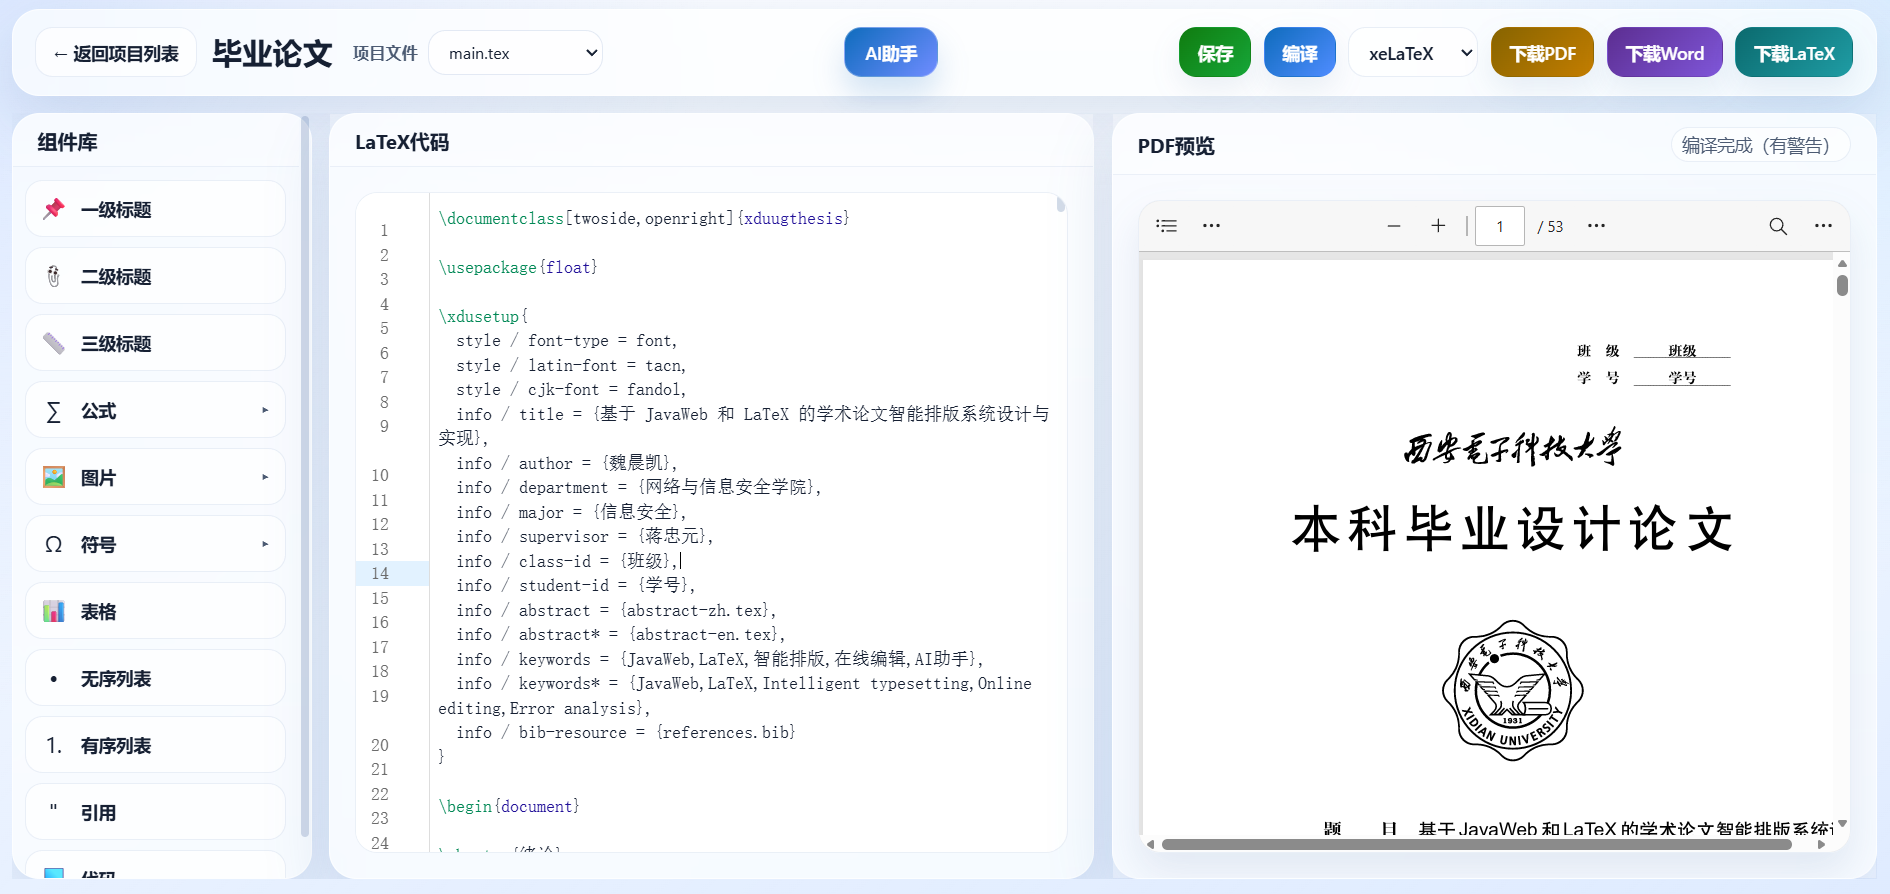
\includegraphics[width=0.75\linewidth]{image.png}
    \caption{AI对话代码片段}
    \label{fig:placeholder}
\end{figure}

\section{核心功能测试}
为了验证系统主要功能是否能够正常运行，本节对核心功能进行简单测试。测试内容包括用户登录、项目创建、LaTeX 编辑保存、论文编译、模板导入和 AI 错误分析等。

\begin{table}[H]
    \centering
    \caption{核心功能测试表}
    \label{tab:core-function-test}
    \begin{tabular}{|c|c|c|c|}
        \hline
        测试编号 & 测试功能 & 测试内容 & 预期结果 \\
        \hline
        T1 & 用户登录 & 输入正确账号和密码 & 登录成功并进入项目列表 \\
        \hline
        T2 & 邮箱验证码 & 输入邮箱并发送验证码 & 邮箱收到验证码 \\
        \hline
        T3 & 创建项目 & 创建空白论文项目 & 项目创建成功并显示在列表中 \\
        \hline
        T4 & 保存论文 & 修改LaTeX内容并保存 & 数据库中项目内容更新 \\
        \hline
        T5 & 模板创建 & 选择模板创建项目 & 项目载入模板初始内容 \\
        \hline
        T6 & LaTeX编译 & 使用xelatex编译论文 & 成功生成PDF \\
        \hline
        T7 & 编译失败反馈 & 输入错误LaTeX语法后编译 & 系统返回错误日志 \\
        \hline
        T8 & AI错误分析 & 对错误日志进行AI分析 & 返回错误原因和修改建议 \\
        \hline
        T9 & PDF导出 & 下载编译生成的PDF & 成功下载PDF文件 \\
        \hline
        T10 & Word导出 & 导出docx文件 & 成功生成Word文件 \\
        \hline
    \end{tabular}
\end{table}

测试结果表明，系统能够完成用户登录、项目管理、在线编辑、模板载入、论文编译、文件导出和 AI 错误分析等主要功能。对于编译失败场景，系统能够返回错误日志，并通过 AI 辅助功能给出相应分析结果，基本满足系统设计目标。

\section{本章小结}
本章对基于 JavaWeb 和 LaTeX 的学术论文智能排版系统进行了详细设计与实现说明。首先介绍了系统开发环境，然后分别对用户管理、论文项目管理、模板管理、LaTeX 在线编辑、论文编译与预览、文件导出和 AI 辅助等核心模块进行了详细阐述，说明了各模块的主要功能、实现流程和关键设计。最后，对系统核心功能进行了测试，验证了系统主要模块能够正常运行。本章内容为后续系统测试和总结分析提供了基础。

\chapter{总结与展望}

\section{总结}
本文围绕《基于JavaWeb和LaTeX的学术论文智能排版系统设计与实现》这一课题，设计并实现了一个面向学术论文写作场景的在线排版系统。系统针对传统论文排版过程中格式调整复杂、LaTeX学习成本较高、模板使用不便以及编译错误难以理解等问题，将论文项目管理、模板管理、LaTeX在线编辑、论文编译、PDF预览、文件导出和AI辅助等功能整合到统一平台中，为用户提供了较为完整的论文写作与排版流程。

在系统设计方面，本文采用前后端分离架构。前端基于Vue 3和Vite实现页面展示与用户交互，后端基于Spring Boot、MyBatis和MySQL实现业务逻辑处理与数据持久化。系统通过接口完成前后端数据交互，并结合token机制实现用户身份认证和权限控制，保证用户能够安全地管理自己的论文项目。

在功能实现方面，系统完成了用户注册登录、邮箱验证码、个人资料管理、论文项目创建与保存、模板载入、管理员zip模板导入、LaTeX源码在线编辑、多引擎编译、PDF预览、Word/LaTeX/PDF导出、AI对话辅助和编译错误分析等功能。其中，LaTeX在线编辑与论文编译是系统的核心功能，用户可以通过浏览器完成论文源码编辑，并使用pdflatex、xelatex、lualatex等编译引擎生成PDF文件。

此外，系统针对LaTeX模板依赖文件较多的问题，在模板导入和编译过程中尽量保留模板目录结构，减少因.cls、.sty、.bib等文件缺失造成的编译失败。同时，系统引入AI辅助功能，在用户遇到LaTeX语法问题或编译错误时，能够提供一定的解释和修改建议，提高了系统的易用性。
通过开发与测试，系统基本实现了预期功能，能够满足用户进行论文在线编辑、模板使用、编译预览和文件导出的基本需求，具有一定的实用价值。

\section{展望}
虽然本系统已经完成了主要功能，但仍存在一些不足，需要在后续继续完善。

首先，系统的模板库仍需扩充。目前系统支持模板导入和载入，但模板数量有限，后续可以增加更多高校毕业论文模板、期刊论文模板和会议论文模板，并为模板提供编译说明和预览效果。

其次，复杂LaTeX模板的兼容性仍有提升空间。部分模板可能依赖特殊宏包、字体文件或多轮编译流程，后续可以增加模板自动检测功能，根据模板内容自动推荐合适的编译引擎和编译方式。

再次，AI辅助功能还可以进一步优化。后续可以结合错误行号、源码上下文和编译日志，提高AI错误分析的准确性，也可以增加LaTeX代码补全、格式检查和自动修改建议等功能。

最后，系统在协作编辑和安全性方面还可以继续增强。后续可以支持多人协同编辑、历史版本管理和导师批注功能；同时加强文件上传校验、编译任务隔离和接口访问控制，提高系统稳定性和安全性。

综上所述，基于JavaWeb和LaTeX的学术论文智能排版系统具有一定应用前景。随着模板库、AI辅助能力、协同编辑能力和安全机制的不断完善，系统能够为用户提供更加便捷、高效的论文写作与排版支持。

\end{document}